%!TEX TS-program = xelatex
\documentclass[12pt, a4paper, oneside]{article}

% пакеты для математики
\usepackage{amsmath,amsfonts,amssymb,amsthm,mathtools}  
\mathtoolsset{showonlyrefs=true}  % Показывать номера только у тех формул, на которые есть \eqref{} в тексте.

\usepackage[british,russian]{babel} % выбор языка для документа
\usepackage[utf8]{inputenc}          % utf8 кодировка

% Основные шрифты 
\usepackage{fontspec}         
\setmainfont{Linux Libertine O}  % задаёт основной шрифт документа

% Математические шрифты 
\usepackage{unicode-math}     
\setmathfont[math-style=upright]{[Neo Euler.otf]} 

%%%%%%%%%% Работа с картинками и таблицами %%%%%%%%%%
\usepackage{graphicx} % Для вставки рисунков                
\usepackage{graphics}
\graphicspath{{images/}{pictures/}}   % папки с картинками

\usepackage[figurename=Картинка]{caption}

\usepackage{wrapfig}    % обтекание рисунков и таблиц текстом

\usepackage{booktabs}   % таблицы как в годных книгах
\usepackage{tabularx}   % новые типы колонок
\usepackage{tabulary}   % и ещё новые типы колонок
\usepackage{float}      % возможность позиционировать объекты в нужном месте
\renewcommand{\arraystretch}{1.2}  % больше расстояние между строками


%%%%%%%%%% Графики и рисование %%%%%%%%%%
\usepackage{tikz, pgfplots}  % языки для графики
%\pgfplotsset{compat=1.16}

\usepackage{todonotes} % для вставки в документ заметок о том, что осталось сделать
% \todo{Здесь надо коэффициенты исправить}
% \missingfigure{Здесь будет Последний день Помпеи}
% \listoftodos --- печатает все поставленные \todo'шки


%%%%%%%%%% Внешний вид страницы %%%%%%%%%%

\usepackage[paper=a4paper, top=20mm, bottom=15mm,left=20mm,right=15mm]{geometry}
\usepackage{indentfirst}    % установка отступа в первом абзаце главы

\usepackage{setspace}
\setstretch{1.15}  % межстрочный интервал
\setlength{\parskip}{4mm}   % Расстояние между абзацами
% Разные длины в LaTeX: https://en.wikibooks.org/wiki/LaTeX/Lengths

% свешиваем пунктуацию
% теперь знаки пунктуации могут вылезать за правую границу текста, при этом текст выглядит ровнее
\usepackage{microtype}

% \flushbottom                            % Эта команда заставляет LaTeX чуть растягивать строки, чтобы получить идеально прямоугольную страницу
\righthyphenmin=2                       % Разрешение переноса двух и более символов
\widowpenalty=300                     % Небольшое наказание за вдовствующую строку (одна строка абзаца на этой странице, остальное --- на следующей)
\clubpenalty=3000                     % Приличное наказание за сиротствующую строку (омерзительно висящая одинокая строка в начале страницы)
\tolerance=10000     % Ещё какое-то наказание.

% мои цвета https://www.artlebedev.ru/colors/
\definecolor{titleblue}{rgb}{0.2,0.4,0.6} 
\definecolor{blue}{rgb}{0.2,0.4,0.6} 
\definecolor{red}{rgb}{1,0,0.2} 
\definecolor{green}{rgb}{0,0.6,0} 
\definecolor{purp}{rgb}{0.4,0,0.8} 

% цвета из geogebra 
\definecolor{litebrown}{rgb}{0.6,0.2,0}
\definecolor{darkbrown}{rgb}{0.75,0.75,0.75}

% Гиперссылки
\usepackage{xcolor}   % разные цвета

\usepackage{hyperref}
\hypersetup{
	unicode=true,           % позволяет использовать юникодные символы
	colorlinks=true,       	% true - цветные ссылки
	urlcolor=blue,          % цвет ссылки на url
	linkcolor=black,          % внутренние ссылки
	citecolor=green,        % на библиографию
	breaklinks              % если ссылка не умещается в одну строку, разбивать её на две части?
}

% меняю оформление секций 
\usepackage{titlesec}
\usepackage{sectsty}

% меняю цвет на синий
\sectionfont{\color{titleblue}}
\subsectionfont{\color{titleblue}}

% выбрасываю нумерацию страниц и колонтитулы 
\pagestyle{empty}

% синие круглые бульпоинты в списках itemize 
\usepackage{enumitem}

\definecolor{itemizeblue}{rgb}{0, 0.45, 0.70}

\newcommand*{\MyPoint}{\tikz \draw [baseline, fill=itemizeblue, draw=blue] circle (2.5pt);}
\renewcommand{\labelitemi}{\MyPoint}

\AddEnumerateCounter{\asbuk}{\@asbuk}{\cyrm}
\renewcommand{\theenumi}{\asbuk{enumi}}

% расстояние в списках
\setlist[itemize]{parsep=0.4em,itemsep=0em,topsep=0ex}
\setlist[enumerate]{parsep=0.4em,itemsep=0em,topsep=0ex}

% эпиграфы
\usepackage{epigraph}
\setlength\epigraphwidth{.6\textwidth}
\setlength\epigraphrule{0pt}

%%%%%%%%%% Свои команды %%%%%%%%%%

% Математические операторы первой необходимости:
\DeclareMathOperator{\sgn}{sign}
\DeclareMathOperator*{\argmin}{arg\,min}
\DeclareMathOperator*{\argmax}{arg\,max}
\DeclareMathOperator{\Cov}{Cov}
\DeclareMathOperator{\Var}{Var}
\DeclareMathOperator{\Corr}{Corr}
\DeclareMathOperator{\E}{\mathop{E}}
\DeclareMathOperator{\Med}{Med}
\DeclareMathOperator{\Mod}{Mod}
\DeclareMathOperator*{\plim}{plim}

% команды пореже
\newcommand{\const}{\mathrm{const}}  % const прямым начертанием
\newcommand{\iid}{\sim i.\,i.\,d.}  % ну вы поняли...
\newcommand{\fr}[2]{\ensuremath{^{#1}/_{#2}}}   % особая дробь
\newcommand{\ind}[1]{\mathbbm{1}_{\{#1\}}} % Индикатор события
\newcommand{\dx}[1]{\,\mathrm{d}#1} % для интеграла: маленький отступ и прямая d

% одеваем шапки на частые штуки
\def \hb{\hat{\beta}}
\def \hs{\hat{s}}
\def \hy{\hat{y}}
\def \hY{\hat{Y}}
\def \he{\hat{\varepsilon}}
\def \hVar{\widehat{\Var}}
\def \hCorr{\widehat{\Corr}}
\def \hCov{\widehat{\Cov}}

% Греческие буквы
\def \a{\alpha}
\def \b{\beta}
\def \t{\tau}
\def \dt{\delta}
\def \e{\varepsilon}
\def \ga{\gamma}
\def \kp{\varkappa}
\def \la{\lambda}
\def \sg{\sigma}
\def \tt{\theta}
\def \Dt{\Delta}
\def \La{\Lambda}
\def \Sg{\Sigma}
\def \Tt{\Theta}
\def \Om{\Omega}
\def \om{\omega}

% Готика
\def \mA{\mathcal{A}}
\def \mB{\mathcal{B}}
\def \mC{\mathcal{C}}
\def \mE{\mathcal{E}}
\def \mF{\mathcal{F}}
\def \mH{\mathcal{H}}
\def \mL{\mathcal{L}}
\def \mN{\mathcal{N}}
\def \mU{\mathcal{U}}
\def \mV{\mathcal{V}}
\def \mW{\mathcal{W}}

% Жирные буквы
\def \mbb{\mathbb}
\def \RR{\mbb R}
\def \NN{\mbb N}
\def \ZZ{\mbb Z}
\def \PP{\mbb{P}}
\def \QQ{\mbb Q}

%%%%%%%%%% Теоремы %%%%%%%%%%
\theoremstyle{plain} % Это стиль по умолчанию.  Есть другие стили.
\newtheorem{theorem}{Теорема}[section]
\newtheorem{result}{Следствие}[theorem]
% счётчик подчиняется теоремному, нумерация идёт по главам согласованно между собой

% убирает курсив и что-то еще наверное делает ;)
\theoremstyle{definition}         
\newtheorem*{definition}{Определение}  % нумерация не идёт вообще


%%%%%%%%%% Задачки и решения %%%%%%%%%%
\usepackage{etoolbox}    % логические операторы для своих макросов
\usepackage{environ}
\newtoggle{lecture}

\newcounter{probNum}[section]  % счётчик для упражнений 
\NewEnviron{problem}[1]{%
    \refstepcounter{probNum}% увеличели номер на 1 
    {\noindent \textbf{\large \color{titleblue} Упражнение~\theprobNum~#1}  \\ \\ \BODY}
    {}%
  }

% Окружение, чтобы можно было убирать решения из pdf
\NewEnviron{sol}{%
  \iftoggle{lecture}
    {\noindent \textbf{\large Решение:} \\ \\ \BODY}
    {}%
  }
 
% выделение по тексту важных вещей
\newcommand{\indef}[1]{\textbf{ \color{green} #1}} 
  
% разные дополнения для картинок
\usetikzlibrary{arrows.meta}
\usepackage{varwidth}

% рисование крестов
% https://tex.stackexchange.com/questions/123760/draw-crosses-in-tikz
\tikzset{
    cross/.pic = {
    \draw[line width=2.pt, rotate = 45] (-#1,0) -- (#1,0);
    \draw[line width=2.pt, rotate = 45] (0,-#1) -- (0, #1);
    }
}
  


\title{Тятя! Тятя! Наши сети притащили мертвеца!}
\date{ }
\author{Ульянкин Филипп}

\begin{document}

% Если переключить в false, все sol исчезнут из pdf
\toggletrue{lecture}
%\togglefalse{lecture}

\maketitle
	
\begin{abstract}
   Однажды вечером Маша читала книгу. 
   
   Благодаря символическому дифференцированию вам никогда не придется заниматься реализацией агоритма обратного распространения вручную. Поэтому не будем тратить время на его формулировку\footnote{Франсуа Шолле, Глубокое обучение на Python, стр. 77}.
   
   Тут ещё пара таких цитат и рофл из Гудфелоу
   
   \indef{Доколе можно такое терпеть?} Если ты не понимаешь как самостоятельно реализовать самую топорную версию модели, а потом ввести в неё несколько простеньких улучшений --- ты не понимаешь эту модель.
    
    % Ты никогда не сможешь сполна проникнуться ей, понять все её прелести, изучить и сполна использовать все её рычажки. Ты никогда не сможешь немного видоизменить её и применить те же самые принципы для новой задачи. Она никогда не будет с тобой искренней. Ты будешь думать, что она показывает свои самые лучшие метрики, в то время, как на самом деле, она будет улыбаться другому. Тому кто знает, где у неё гиперпараметр $G$.
    
    % Как понять внутренности и суметь написать код, описывающий их? Как заслужить её любовь и искренность? Надо окунаться в математику, которая за ней стоит. Однако она иногда бывает слишком сложной. Это отбивает всё желание быть с ней полностью на одной волне. 
    
    % Эта серия виньеток сделана для тех, кто хочет не просто поиграться с прелестями машинного обучения. Она для тех, кто хочет досконально их прочувствовать. Через серию инфантильных задачек мы будем идти от простых вещей к сложным до тех пор, пока не окажемся на пике. 
    
    % Здесь и сегодня пойдёт речь о нейронных сетках. Мы попробуем понять как работает Backpropagation ручками на бумажке. Шаг за шагом, .... 
    
    % Послать тут всех хейтеров нахрен и написать что это не дип лернинг от бенджи и ко, а инфантильные задачи на пару вечеров
    \todo[inline]{Написать по-нормальному abstract!}
\end{abstract}
	
\tableofcontents

\todo[inline]{Все должно быть в концепте маши кому принадлежит лёрнинг, все задачки должны ложиться в историю про неё, решения должны быть органично оторваны от личности Маши.}
	
\section{Всего лишь функция} 

\epigraph{Ты всего лишь машина, только имитация жизни. Робот сочинит симфонию? Робот превратит кусок холста в шедевр искусства?}{Из фильма <<Я, робот>> (2004)}

\begin{problem}{(от регрессии к нейросети)}
Маша зашла в свою любимую кофейню на Тверской выпить кофе. На стене кофейни она увидела интересную картину:

\begin{center}
\begin{tikzpicture}[line cap=round,line join=round,x=1.0cm,y=1.0cm]

\draw [line width=1.pt] (0,1.5) circle (0.5cm) node {$1$};
\draw [line width=1.pt] (2,1.5) circle (0.5cm) node {$x$};
\draw [line width=1.pt] (1,-1) circle (0.5cm) node {$\hat y$};

\draw [->, line width=1.pt] (0,1) -- (0.9,-0.4) node[pos=0.3,right] {\small $w_1$};
\draw [->, line width=1.pt] (2,1) -- (1.1,-0.4) node[pos=0.3,left] {\small $w_2$};
\end{tikzpicture}
\end{center}


Хозяин кофейни Добродум объяснил Маше, что это модель 


А потом короч типа 

\begin{center}
\begin{tikzpicture}[line cap=round,line join=round,x=1.0cm,y=1.0cm]

\draw [line width=1.pt] (0,2.5) circle (0.5cm) node {$1$};
\draw [line width=1.pt] (2,2.5) circle (0.5cm) node {$x$};

\draw [line width=1.pt] (0,-0.5) circle (0.5cm) node {$h_1$};
\draw [line width=1.pt] (2,-0.5) circle (0.5cm) node {$h_2$};

\draw [line width=1.pt] (1,-3) circle (0.5cm) node {$\hat y$};

\draw [->, line width=1.pt] (0,2) -- (-0.1,0.1) node[pos=0.3,left] {\small $w_{11}$};
\draw [->, line width=1.pt] (2,2) -- (2.1,0.1) node[pos=0.3,right] {\small $w_{22}$};

\draw [->, line width=1.pt] (0,2) -- (1.9,0.1) node[pos=0.5,left] {\small $w_{12}$};
\draw [->, line width=1.pt] (2,2) -- (0.1,0.1) node[pos=0.5,right] {\small $w_{21}$};

\draw [->, line width=1.pt] (0,-1) -- (0.8,-2.4) node[pos=0.3,right] {\small $w_{1}$};
\draw [->, line width=1.pt] (2,-1) -- (1.2,-2.4) node[pos=0.3,left] {\small $w_{2}$};
\end{tikzpicture}
\end{center}



Тут лёгкая задачка про то как регрессия превращается в нейронку + пункт про то что без функции активации будет то же самое на примере 2 регрессоров
\end{problem}

\begin{sol}
А тут решение :) 
\end{sol} 


\begin{problem}{(из картинки в формулу)}
Добродум хозяин кофейни на Тверской. Он хочет понять насколько сильно будет заполнена кофейня в следующие выходные. Для этого по старым данным он обучил нейросетку. На вход она принимает три фактора: температуру за окном, $x_1$, факт наличия на Тверской митинга, $x_2$ и пол баристы на смене, $x_3$.  В качестве функции активации Добродум использует $ReLU.$ 

\begin{center}
\begin{tikzpicture}[line cap=round,line join=round,x=1.0cm,y=1.0cm]

\draw [line width=1.pt] (-3,1.5) circle (0.5cm) node {$x_1$};
\draw [line width=1.pt] (-3,-0.5) circle (0.5cm) node {$x_2$};
\draw [line width=1.pt] (-3,-2.5) circle (0.5cm) node {$x_3$};	

\draw [line width=1.pt] (-1,0)--(1,0)--(1,1)--(-1,1)--cycle;
\draw (0,0.5) node {$f(h)$};
\draw [line width=1.pt] (-1,-2)--(1,-2)--(1,-1)--(-1,-1)--cycle;
\draw (0,-1.5) node {$f(h)$};

\draw [line width=1.pt] (3,1.5) circle (0.5cm) node {$1$};	
\draw [line width=1.pt] (2,-1)--(4,-1)--(4,0)--(2,0)--cycle;
\draw (3,-0.5) node {$f(h)$};

\draw [line width=1.pt] (-2.5,1.5) -- (-1,0.5) node[pos=0.5,above] {\small $5$};
\draw [line width=1.pt] (-2.5,1.5) -- (-1,-1.5) node[pos=0.3,left] {\small $-2$};
\draw [line width=1.pt] (-2.5,-0.5) -- (-1,0.5) node[pos=0.5,left] {\small $-60$};
\draw [line width=1.pt] (-2.5,-0.5) -- (-1,-1.5)  node[pos=0.5,left] {\small  $-80$};
\draw [line width=1.pt] (-2.5,-2.5) -- (-1,0.5) node[near start,left] {\small $0.5$};
\draw [line width=1.pt] (-2.5,-2.5) -- (-1,-1.5)  node[near start,below] {\small  $2$};

\draw [line width=1.pt] (1,0.5) -- (2,-0.5) node[pos=0.25,right] {\small $1$};
\draw [line width=1.pt] (1,-1.5) -- (2,-0.5) node[pos=0.2,right] {\small $0.2$};
\draw [line width=1.pt] (3,1) -- (3,0) node[pos=0.5,right] {\small  $4$};

\draw [->] (4,-0.5) -- (5,-0.5) node[right] {$\hat y$};
\end{tikzpicture}
\end{center}

\begin{enumerate}
\item В эти выходные за барной стойкой стоит Агнесса. Митинга не предвидится, температура будет в районе $20$ градусов. Сколько человек придёт в кофейню к Добродуму? 

\item На самом деле каждая нейросетка --- это просто-напросто какая-то нелинейная сложная функция. Запишите нейросеть Добродума в виде функции.
\end{enumerate}
\end{problem}

\begin{sol}
Будем постепенно идти по сетке и делать вычисления. Подаём все значения в первый нейрон, получаем: 

$$
h_1 = \max(0, 5 \cdot 20 + (-60) \cdot 0 + 0.5 \cdot 1) = \max(0, 100.5) = 100.5
$$

Ровно то же самое делаем со вторым нейроном: 

$$
h_2 = \max(0, -2 \cdot 20 + (-80) \cdot 0 + 2 \cdot 1) = \max(0, -38) = 0
$$

Дальше результат скрытых нейронов идёт во второй слой: 

$$
\hat y = \max(0, 1 \cdot 100.5 + 0.2 \cdot 0 + 4 \cdot 1) = 104.5
$$

Это и есть итоговый прогноз.

\begin{center}
\begin{tikzpicture}[line cap=round,line join=round,x=1.0cm,y=1.0cm]

\draw [line width=1.pt] (-3,1.5) circle (0.5cm) node {$20$};
\draw [line width=1.pt] (-3,-0.5) circle (0.5cm) node {$0$};
\draw [line width=1.pt] (-3,-2.5) circle (0.5cm) node {$1$};	

\draw [line width=1.pt] (-1,0)--(1,0)--(1,1)--(-1,1)--cycle;
\draw (0,0.5) node {$100.5$};
\draw [line width=1.pt] (-1,-2)--(1,-2)--(1,-1)--(-1,-1)--cycle;
\draw (0,-1.5) node {$0$};

\draw [line width=1.pt] (3,1.5) circle (0.5cm) node {$1$};	
\draw [line width=1.pt] (2,-1)--(4,-1)--(4,0)--(2,0)--cycle;
\draw (3,-0.5) node {$104.5$};

\draw [line width=1.pt] (-2.5,1.5) -- (-1,0.5) node[pos=0.5,above] {\small $5$};
\draw [line width=1.pt] (-2.5,1.5) -- (-1,-1.5) node[pos=0.3,left] {\small $-2$};
\draw [line width=1.pt] (-2.5,-0.5) -- (-1,0.5) node[pos=0.5,left] {\small $-60$};
\draw [line width=1.pt] (-2.5,-0.5) -- (-1,-1.5)  node[pos=0.5,left] {\small  $-80$};
\draw [line width=1.pt] (-2.5,-2.5) -- (-1,0.5) node[near start,left] {\small $0.5$};
\draw [line width=1.pt] (-2.5,-2.5) -- (-1,-1.5)  node[near start,below] {\small  $2$};

\draw [line width=1.pt] (1,0.5) -- (2,-0.5) node[pos=0.25,right] {\small $1$};
\draw [line width=1.pt] (1,-1.5) -- (2,-0.5) node[pos=0.2,right] {\small $0.2$};
\draw [line width=1.pt] (3,1) -- (3,0) node[pos=0.5,right] {\small  $4$};

\draw [->] (4,-0.5) -- (5,-0.5) node[right] {$\hat y$};
\end{tikzpicture}
\end{center}

Теперь по мотивам наших вычислений запишем нейронку как функцию. Начинать будем с конца:

$$
\hat y = f(1 \cdot h_1 + 0.2 \cdot h_2 + 4 \cdot 1)
$$

Подставляем вместо $h_1$ и $h_2$ вычисления, которые происходят на первом слое нейронки: 

\begin{multline*}
\hat y = f(1 \cdot f(5 \cdot x_1 -60 \cdot x_2 + 0.5 \cdot x_3) + 0.2 \cdot f(-2 \cdot x_1 -80 \cdot x_2 + 2 \cdot x_3) + 4 \cdot 1) = \\ = \max(0, \max(0, 5 \cdot x_1 -60 \cdot x_2 + 0.5 \cdot x_3) + 0.2 \cdot \max(0, -2 \cdot x_1 -80 \cdot x_2 + 2 \cdot x_3) + 4).
\end{multline*}

Обучение нейронной сетки на самом деле эквивалентно обучению такой сложной нелинейной функции. 
\end{sol}


%%%-------------------------------------------
\begin{problem}{(из формулы в картинку)}
Теперь в обратную сторону. Пусть у нас есть вот такая функция. 
\[
y = \max(0, 4 \cdot \max(0, 3 \cdot x_1 + 4 \cdot x_2 + 1) + 2 \cdot \max(0, 3 \cdot x_1 + 2 \cdot x_2 + 7) + 6)
\]

Нарисуйте эту функцию в виде нейросетки.
\end{problem}

\begin{sol}
Начнём рисовать картинку с конца. На выход выплёвывается либо $0$, либо комбинация из двух входов: 

$$
\hat y = ReLU(4 \cdot h_1 + 2 \cdot h_2 + 6)
$$

Каждый из входов --- это снова либо $0$, либо комбинация из двух входов. 

$$
y = \max(0, {\color{red} 4} \cdot \underbrace{\max(0, 3 \cdot x_1 +  4 \cdot x_2 + 1)}_{h_1} + {\color{red} 2} \cdot \underbrace{\max(0, {\color{purp} 3} \cdot x_1 + {\color{purp} 2} \cdot x_2 + {\color{purp} 7})}_{h_2} + {\color{red} 6})
$$

Получается, что на первом слое находится два нейрона, которые передают свои выходы в третий:

\begin{center}
\begin{tikzpicture}[line cap=round,line join=round,x=1.0cm,y=1.0cm]

\draw [line width=1.pt] (-3,1.5) circle (0.5cm) node {$1$};
\draw [line width=1.pt] (-3,-0.5) circle (0.5cm) node {$x_1$};
\draw [line width=1.pt] (-3,-2.5) circle (0.5cm) node {$x_2$};	

\draw [line width=1.pt] (-1,0)--(1,0)--(1,1)--(-1,1)--cycle;
\draw (0,0.5) node {$ReLU$};
\draw (1,1) node[right] {$h_1$};
\draw [line width=1.pt] (-1,-2)--(1,-2)--(1,-1)--(-1,-1)--cycle;
\draw (0,-1.5) node {$ReLU$};
\draw (1,-2) node[right] {$h_2$};

\draw [line width=1.pt] (3,1.5) circle (0.5cm) node {$1$};	
\draw [line width=1.pt] (2,-1)--(4,-1)--(4,0)--(2,0)--cycle;
\draw (3,-0.5) node {$ReLU$};

\draw [line width=1.pt] (-2.5,1.5) -- (-1,0.5) node[near start,above] {\small $1$};
\draw [line width=1.pt, purp] (-2.5,1.5) -- (-1,-1.5) node[near start,right] {\small \color{purp} $7$};
\draw [line width=1.pt] (-2.5,-0.5) -- (-1,0.5) node[near start,above] {\small $3$};
\draw [line width=1.pt, purp] (-2.5,-0.5) -- (-1,-1.5)  node[near start,above] {\small \color{purp} $3$};
\draw [line width=1.pt] (-2.5,-2.5) -- (-1,0.5) node[near start,left] {\small $4$};
\draw [line width=1.pt, purp] (-2.5,-2.5) -- (-1,-1.5)  node[near start,below] {\small \color{purp} $2$};

\draw [line width=1.pt, red] (1,0.5) -- (2,-0.5) node[pos=0.5,above] {\small \color{red} $4$};
\draw [line width=1.pt, red] (1,-1.5) -- (2,-0.5) node[pos=0.5,below] {\small \color{red} $2$};
\draw [line width=1.pt, red] (3,1) -- (3,0) node[pos=0.5,right] {\small \color{red} $6$};

\draw [->] (4,-0.5) -- (5,-0.5) node[right] {$\hat y$};
\end{tikzpicture}
\end{center}
\end{sol}


%%%-------------------------------------------
\begin{problem}{(армия регрессий)}
Парни очень любят Машу, а Маша с недавних пор любит собирать перcептроны и думать по вечерам об их весах и функциях активации. Сегодня она решила разобрать свои залежи из перcептронов и как следует упорядочить их. 

\begin{enumerate}

\item В ящике стола Маша нашла перcептрон с картинки \ref{perp1} Маша хочет подобрать веса так, чтобы он реализовывал логическое отрицание, то есть превращал $x_1 = 0$ в $y=1$, а $x_1 = 1$ в $y=0$.

\begin{minipage}{0.49\linewidth}
\begin{figure}[H]
\caption{} \label{perp1}
\begin{center}
\begin{tikzpicture}[line cap=round,line join=round,x=1.0cm,y=1.0cm]
\clip(-4,0) rectangle (3,4.5); % чтобы выравнять картинки по размерам
\draw [line width=1.pt] (-3,4) circle (0.5cm) node {$1$};
\draw [line width=1.pt] (-3,2) circle (0.5cm) node {$x_1$};

\draw [line width=1.pt] (-1,3.5)--(-1,2.5)--(1.5,2.5)-- (1.5,3.5) -- cycle;

\draw [->, line width=1.pt] (-2.5,4) -- (-1.1,3.1) node[pos=0.3,above] {\small $w_1$};
\draw [->, line width=1.pt] (-2.5,2) -- (-1.1,2.9) node[pos=0.3,above] {\small $w_2$};
\draw [->, line width=1.pt] (1.5,3) -- (2.5,3) node[pos=1,right] {$\hat y$};
\draw (0.3,3) node {$\max(0,h)$};
\end{tikzpicture}
\end{center}
\end{figure}
\end{minipage}
\hfill
\begin{minipage}{0.49\linewidth}
\begin{figure}[H]
\caption{} \label{perp2}
\begin{center}
\begin{tikzpicture}[line cap=round,line join=round,x=1.0cm,y=1.0cm]
\clip(-4,0) rectangle (3,4.5);
\draw [line width=1.pt] (-3,4) circle (0.5cm) node {$x_1$};
\draw [line width=1.pt] (-3,2.5) circle (0.5cm) node {$x_2$};
\draw [line width=1.pt] (-3,1) circle (0.5cm) node {$x_3$};

\draw [line width=1.pt] (-1,3)--(-1,2)--(1.5,2)--(1.5,3)--cycle;
\draw (0.3,2.5) node {$\max(0,h)$};

\draw [->, line width=1.pt] (-2.5,4)--(-1.1,2.7) node[pos=0.5,above] {\small $w_1$};
\draw [->, line width=1.pt] (-2.5,2.5)--(-1.1,2.5) node[pos=0.3,above] {\small $w_2$};
\draw [->, line width=1.pt] (-2.5,1)--(-1.1,2.3) node[pos=0.5,below] {\small $w_3$};
\draw [->, line width=1.pt] (1.5,2.5)--(2.5,2.5) node[pos=1,right] {$\hat y$};
\end{tikzpicture}
\end{center}
\end{figure}
\end{minipage}

\item В тумбочке среди носков Маша нашла перcептрон, с картинки \ref{perp2}, Маша хочет подобрать такие веса $w_i$, чтобы персептрон превращал $x$ из таблички в соответствующие $y$:
	
\begin{center}
	\begin{tabular}{c|c|c|c}
    	$x_1$ & $x_2$ & $x_3$ & $y$ \\
    	\hline 
    	$1$ & $1$ & $2$ & $0.5$\\
    	\hline 
    	$1$ & $-1$ & $1$ & $0$ \\
	\end{tabular}
\end{center}

\item Оказывается, что в ванной всё это время валялась куча персептронов с картинки \ref{perp3} с неизвестной функцией активации (надо самому выбирать). 

\begin{minipage}{0.49\linewidth}
\begin{figure}[H]
\caption{} \label{perp3}
\begin{center}
\begin{tikzpicture}[line cap=round,line join=round,x=1.0cm,y=1.0cm]
\clip(-4,0) rectangle (3,4.5);
\draw [line width=1.pt] (-3,4) circle (0.5cm) node {$1$};
\draw [line width=1.pt] (-3,2.5) circle (0.5cm) node {$x_1$};
\draw [line width=1.pt] (-3,1) circle (0.5cm) node {$x_2$};

\draw [line width=1.pt] (-1,3)--(-1,2)--(1.5,2)--(1.5,3)--cycle;
\draw (0.3,2.5) node {$f(h)$};

\draw [->, line width=1.pt] (-2.5,4)--(-1.1,2.7) node[pos=0.5,above] {\small $w_1$};
\draw [->, line width=1.pt] (-2.5,2.5)--(-1.1,2.5) node[pos=0.3,above] {\small $w_2$};
\draw [->, line width=1.pt] (-2.5,1)--(-1.1,2.3) node[pos=0.5,below] {\small $w_3$};
\draw [->, line width=1.pt] (1.5,2.5)--(2.5,2.5) node[pos=1,right] {$\hat y$};
\end{tikzpicture}
\end{center}
\end{figure}
\end{minipage}
\hfill
\begin{minipage}{0.49\linewidth}
\begin{figure}[H]
\caption{} \label{perp4}
\begin{center}
	\begin{tikzpicture}[line cap=round,line join=round,x=1.0cm,y=1.0cm]
	\clip(-2,-5) rectangle (4,-0.5);
	\draw [->,line width=2.pt] (1,-5) -- (1,-1);
	\draw [->,line width=2.pt] (-2,-3) -- (4,-3);
	\draw (2,-1.25) node[anchor=north west] {$1$};
	\draw (-0.3,-2.4) node[anchor=north west] {$0$};
	\draw (1.9,-4) node[anchor=north west] {$0$};
	\draw (3.2,-2.5) node[anchor=north west] {$0$};	
	\draw [line width=2.pt,dash pattern=on 3pt off 3pt] (0,-5)-- (4,-1);
	\draw [line width=2.pt,dash pattern=on 3pt off 3pt] (0,-1)-- (4,-5);
	\end{tikzpicture}
\end{center}
\end{figure}
\end{minipage}

Маша провела на плоскости две прямые: $x_1 + x_2 = 1$ и $x_1 - x_2 = 1$. Она хочет собрать из персептронов нейросетку, которая будет классифицировать объекты с плоскости так, как показано на картинке \ref{perp4}.

\item В коробке на кухне завалялось три персептрона, у каждого два входа с константой и пороговая функция активации. Маша хочет реализовать с их помощью функцию

$$
y = \begin{cases}
1, \text{ если } x_2 \geq |x_1 - 3| + 2; \\
0, \text{ иначе}
\end{cases}.
$$
\end{enumerate}
\end{problem}

\begin{sol}
\begin{enumerate}
\item Начнём с первого пункта. Чтобы было легче запишем нейрон в виде уравнения: 

$$
\hat y = \max(0, w_1 + w_2 \cdot x_1).
$$

Нам нужно, чтобы 

\begin{equation*}
\begin{aligned}
\max(0, w_1 + w_2 \cdot 1) = 0 \\ 
\max(0, w_1 + w_2 \cdot 0) = 1 
\end{aligned}
\end{equation*}

Из второго уравнения сразу получаем, что $w_1 = 1$, а $w_2$ на второе уравнение никак не влияет. Для того, чтобы в первом уравнении получить ноль, нужно взять $w_2 \le -1$. Нейрон готов. 

\item Снова выписываем несколько уравнений: 

\begin{equation*}
\begin{aligned}
\max(0, w_1 + w_2 + 2 \cdot w_3) = 0.5 \\ 
\max(0, w_1 - w_2 + w_3) = 0 
\end{aligned}
\end{equation*}

Тут решений может быть довольно много. Первое, что приходит в голову --- это занулить $w_1$ и $w_3$ в первом уравнении, а $w_2$ поставить $0.5$. Тогда во втором уравнении мы сразу же будем оказываться в отрицательной области и $ReLU$ заботливо будет отдавать нам $0$. 

\item Давайте для разнообразия возьмём в качестве $f(h)$ пороговую функцию потерь

$$
f(h) = \begin{cases} 1, h > 0 \\ 0, h \le 0 \end{cases}.
$$

Один нейрон --- это одна линия, проведённая на плоскости. Эта линия отделяет один класс от другого. Например, линию $ x_1 + x_2 - 1 = 0 $ мог бы описать нейрон 

\begin{minipage}{0.49\linewidth}
\begin{center}
\begin{tikzpicture}[line cap=round,line join=round,x=1.0cm,y=1.0cm]
\clip(-4,0) rectangle (3.5,4.5);
\draw [line width=1.pt] (-3,4) circle (0.5cm) node {$1$};
\draw [line width=1.pt] (-3,2.5) circle (0.5cm) node {$x_1$};
\draw [line width=1.pt] (-3,1) circle (0.5cm) node {$x_2$};

\draw [line width=1.pt] (-1,3)--(-1,2)--(1.5,2)--(1.5,3)--cycle;
\draw [line width=1.pt] (-0.6,2.2)--(0.2,2.2)--(0.2,2.8)--(1,2.8);
\draw (0.3,1.7) node {$\gamma = 0$};

\draw [->, line width=1.pt] (-2.5,4)--(-1.1,2.7) node[pos=0.5,above] {\small $-1$};
\draw [->, line width=1.pt] (-2.5,2.5)--(-1.1,2.5) node[pos=0.3,above] {\small $1$};
\draw [->, line width=1.pt] (-2.5,1)--(-1.1,2.3) node[pos=0.5,below] {\small $1$};
\draw [->, line width=1.pt] (1.5,2.5)--(2.5,2.5) node[pos=1,right] {$h_1$};
\end{tikzpicture}
\end{center}
\end{minipage}
\hfill
\begin{minipage}{0.49\linewidth}
\begin{center}
	\begin{tikzpicture}[line cap=round,line join=round,x=1.0cm,y=1.0cm]
	\clip(0,-5) rectangle (4,-0.5);
 	\draw (2,-1.25) node[anchor=north west] {$1$};
 	\draw (0.3,-2.4) node[anchor=north west] {$0$};
	\draw [line width=2.pt,dash pattern=on 3pt off 3pt] (0,-1)-- (4,-5);
	\end{tikzpicture}
\end{center}
\end{minipage}

Порог $\gamma$ для кусочной функции в каком-то смысле дублирует константу. Будем всегда брать его нулевым. Видим, что если мы получили комбинацию $x_1$, $x_2$ и $1$, большую, чем ноль, мы оказались справа от прямой. Если хочется поменять метку $0$ и $1$ сторонами, можно умножить все коэффициенты на $-1$. \indef{Наш персептрон понимает по какую сторону от прямой мы оказались,} то есть задаёт одну линейную разделяющую поверхность.  По аналогии для второй прямой мы можем получить: 

\begin{minipage}{0.49\linewidth}
\begin{center}
\begin{tikzpicture}[line cap=round,line join=round,x=1.0cm,y=1.0cm]
\clip(-4,0) rectangle (3.5,4.5);
\draw [line width=1.pt] (-3,4) circle (0.5cm) node {$1$};
\draw [line width=1.pt] (-3,2.5) circle (0.5cm) node {$x_1$};
\draw [line width=1.pt] (-3,1) circle (0.5cm) node {$x_2$};

\draw [line width=1.pt] (-1,3)--(-1,2)--(1.5,2)--(1.5,3)--cycle;
\draw [line width=1.pt] (-0.6,2.2)--(0.2,2.2)--(0.2,2.8)--(1,2.8);
\draw (0.3,1.7) node {$\gamma = 0$};

\draw [->, line width=1.pt] (-2.5,4)--(-1.1,2.7) node[pos=0.5,above] {\small $1$};
\draw [->, line width=1.pt] (-2.5,2.5)--(-1.1,2.5) node[pos=0.3,above] {\small $-1$};
\draw [->, line width=1.pt] (-2.5,1)--(-1.1,2.3) node[pos=0.5,below] {\small $1$};
\draw [->, line width=1.pt] (1.5,2.5)--(2.5,2.5) node[pos=1,right] {$h_2$};
\end{tikzpicture}
\end{center}
\end{minipage}
\hfill
\begin{minipage}{0.49\linewidth}
\begin{center}
	\begin{tikzpicture}[line cap=round,line join=round,x=1.0cm,y=1.0cm]
	\clip(0,-5) rectangle (4,-0.5);
 	\draw (2,-1.25) node[anchor=north west] {$1$};
 	\draw (1.9,-4) node[anchor=north west] {$0$};
 	\draw [line width=2.pt,dash pattern=on 3pt off 3pt] (0,-5)-- (4,-1);
	\end{tikzpicture}
\end{center}
\end{minipage}

Итак, первый персептрон выбрал нам позицию относительно первой прямой, второй относительно второй. Остаётся только соединить эти результаты в один. Нейрон для скрепки должен реализовать для нас логическую функцию, которую задаёт табличка ниже. Там же нарисованы примеры весов, которые могли бы объединить выхлоп первого слоя в итоговый прогноз.

\begin{minipage}{0.1\linewidth}
\begin{center}
\begin{tabular}{c|c|c}
	$h_1$ & $h_2$ & $\hat y$ \\
	\hline 
	$1$ & $1$ & {\color{green} $1$} \\
	\hline 
	$1$ & $0$ & {\color{green} $0$} \\
	\hline 
	$0$ & $1$ & {\color{green} $0$} \\
	\hline 
	$0$ & $0$ & {\color{green} $0$} \\
\end{tabular}
\end{center}
\end{minipage}
\hfill
\begin{minipage}{0.44\linewidth}
\begin{center}
	\begin{tikzpicture}[line cap=round,line join=round,x=1.0cm,y=1.0cm]
	\clip(-2,-5) rectangle (4,-0.5);
	
	\draw (2,-1.9) node[anchor=north west] {\color{green} $1$};
	\draw (1.6,-1.1) node[anchor=north west] {$(1, 1)$};
	
	\draw (-0.3,-2.2) node[anchor=north west] {\color{green} $0$};
	\draw (-0.7,-3) node[anchor=north west] {$(0, 1)$};
	
	\draw (1.9,-3.5) node[anchor=north west] {\color{green} $0$};
	\draw (1.5,-4.2) node[anchor=north west] {$(0, 0)$};
	
	\draw (3.2,-2.2) node[anchor=north west] {\color{green} $0$};	
	\draw (2.9,-2.8) node[anchor=north west] {$(1, 0)$};	
	
	\draw [line width=2.pt,dash pattern=on 3pt off 3pt] (0,-5)-- (4,-1);
	\draw [line width=2.pt,dash pattern=on 3pt off 3pt] (0,-1)-- (4,-5);
	\end{tikzpicture}
\end{center}
\end{minipage}
\hfill
\begin{minipage}{0.44\linewidth}
\begin{center}
\begin{tikzpicture}[line cap=round,line join=round,x=1.0cm,y=1.0cm]
\clip(-4,0) rectangle (3,4.5);
\draw [line width=1.pt] (-3,4) circle (0.5cm) node {$1$};
\draw [line width=1.pt] (-3,2.5) circle (0.5cm) node {$h_1$};
\draw [line width=1.pt] (-3,1) circle (0.5cm) node {$h_2$};

\draw [line width=1.pt] (-1,3)--(-1,2)--(1.5,2)--(1.5,3)--cycle;
\draw [line width=1.pt] (-0.6,2.2)--(0.2,2.2)--(0.2,2.8)--(1,2.8);
\draw (0.3,1.7) node {$\gamma = 0$};

\draw [->, line width=1.pt] (-2.5,4)--(-1.1,2.7) node[pos=0.5,above] {\small $-1$};
\draw [->, line width=1.pt] (-2.5,2.5)--(-1.1,2.5) node[pos=0.3,above] {\small $1$};
\draw [->, line width=1.pt] (-2.5,1)--(-1.1,2.3) node[pos=0.5,below] {\small $1$};
\draw [->, line width=1.pt] (1.5,2.5)--(2.5,2.5) node[pos=1,right] {$\hat y$};
\end{tikzpicture}
\end{center}
\end{minipage}

Теперь мы можем нарисовать итоговую нейронную сеть, решающую задачу Маши. Она состоит из двух слоёв. Меньше не выйдет, так как каждый персептрон строит только одну разделяющую линию. 

\begin{center}
\begin{tikzpicture}[line cap=round,line join=round,x=1.0cm,y=1.0cm]

\draw [line width=1.pt] (-3,1.5) circle (0.5cm) node {$1$};
\draw [line width=1.pt] (-3,-0.5) circle (0.5cm) node {$x_1$};
\draw [line width=1.pt] (-3,-2.5) circle (0.5cm) node {$x_2$};	

\draw [line width=1.pt] (-1,0)--(1,0)--(1,1)--(-1,1)--cycle;
\draw [line width=1.pt] (-0.7,0.2)--(0,0.2)--(0,0.8)--(0.7,0.8);
\draw (0,-0.2) node {$\gamma = 0$};

\draw [line width=1.pt] (-1,-2)--(1,-2)--(1,-1)--(-1,-1)--cycle;
\draw [line width=1.pt] (-0.7,-1.8)--(0,-1.8)--(0,-1.2)--(0.7,-1.2);
\draw (0,-2.2) node {$\gamma = 0$};

\draw [line width=1.pt] (3,1.5) circle (0.5cm) node {$1$};	
\draw [line width=1.pt] (2,-1)--(4,-1)--(4,0)--(2,0)--cycle;
\draw [line width=1.pt] (2.3,-0.8)--(3,-0.8)--(3,-0.2)--(3.7,-0.2);
\draw (3,-1.2) node {$\gamma = 0$};

\draw [line width=1.pt] (-2.5,1.5) -- (-1,0.5) node[pos=0.5,above] {\small $-1$};
\draw [line width=1.pt] (-2.5,1.5) -- (-1,-1.5) node[pos=0.3,left] {\small $1$};
\draw [line width=1.pt] (-2.5,-0.5) -- (-1,0.5) node[pos=0.5,left] {\small $1$};
\draw [line width=1.pt] (-2.5,-0.5) -- (-1,-1.5)  node[pos=0.5,left] {\small  $-1$};
\draw [line width=1.pt] (-2.5,-2.5) -- (-1,0.5) node[near start,left] {\small $1$};
\draw [line width=1.pt] (-2.5,-2.5) -- (-1,-1.5)  node[near start,below] {\small  $1$};

\draw [line width=1.pt] (1,0.5) -- (2,-0.5) node[pos=0.25,right] {\small $1$};
\draw [line width=1.pt] (1,-1.5) -- (2,-0.5) node[pos=0.2,right] {\small $1$};
\draw [line width=1.pt] (3,1) -- (3,0) node[pos=0.5,right] {\small  $-1$};

\draw [->] (4,-0.5) -- (5,-0.5) node[right] {$\hat y$};
\end{tikzpicture}
\end{center}

Кстати говоря, если бы мы ввели для нашей нейросетки дополнительный признак $x_1 \cdot x_2$, у нас бы получилось обойтись только одним персептроном. В нашей ситуации \indef{нейросетка сама сварила на первом слое признак $x_1 \cdot x_2$, которого ей не хватало.} 

\item  \todo[inline]{Вбить решение}
\end{enumerate}
\end{sol}


%%%-------------------------------------------
\begin{problem}{(логические функции)}
Есть теорема, которая говорит о том, что с помощью нейросетки можно аппроксимировать почти любую функцию. Попробуйте с помощью нейросеток с минимально возможным числом нейронов описать логический функции, заданные следующими таблицами истинности:

\begin{center}
\begin{minipage}{0.3\linewidth} 
\begin{tabular}{c|c|c}
	$x_1$ & $x_2$ & $x_1 \cap x_2$ \\
	\hline 
	$1$ & $1$ & $1$ \\
	\hline 
	$1$ & $0$ & $0$ \\
	\hline 
	$0$ & $1$ & $0$ \\
	\hline 
	$0$ & $0$ & $0$ \\
\end{tabular}
\end{minipage}
\hfill
\begin{minipage}{0.3\linewidth}
		\begin{tabular}{c|c|c}
		$x_1$ & $x_2$ & $x_1 \cup x_2$ \\
		\hline 
		$1$ & $1$ & $1$ \\
		\hline 
		$1$ & $0$ & $1$ \\
		\hline 
		$0$ & $1$ & $1$ \\
		\hline 
		$0$ & $0$ & $0$ \\
	\end{tabular}
\end{minipage}
\hfill
\begin{minipage}{0.3\linewidth}
		\begin{tabular}{c|c|c}
		$x_1$ & $x_2$ & $x_1 \mbox{ } XoR \mbox{ } x_2$ \\
		\hline 
		$1$ & $1$ & $0$ \\
		\hline 
		$1$ & $0$ & $1$ \\
		\hline 
		$0$ & $1$ & $1$ \\
		\hline 
		$0$ & $0$ & $0$ \\
	\end{tabular}
\end{minipage}
\end{center}

Первые два столбика идут на вход, третий получается на выходе.  Операция из третьей таблицы называется исключающим или (XoR). Если внимательно приглядеться, то можно заметить, что $XoR$ --- это то же самое что и $[x_1 \ne x_2]$\footnote{Тут квадратные скобки обозначают индикатор. Он выдаёт $1$, если внутри него стоит правда и $0$, если ложь.}. 
\end{problem}

\begin{sol} 
На самом деле в предыдущем упражнении мы уже построили нейрон для пересечения, когда нам нужно было оказаться два раза по правильную сторону прямой. Посмотрим на тот же нейрон под другим углом:

\begin{minipage}{0.29\linewidth}
\begin{center}
	\begin{tikzpicture}[line cap=round,line join=round,x=1.0cm,y=1.0cm]
    
    \draw [->, line width=1.pt] (-0.3,0) --(3.5,0); 
    \draw [->, line width=1.pt] (0,-0.3) --(0,3.5); 
    
    \draw [fill=blue] (0,0) circle (4pt);
    \draw [fill=blue] (0,2) circle (4pt);
    \draw [fill=blue] (2,0) circle (4pt);
    \path (2,2) pic[red] {cross=4pt};
    \draw [line width=2.pt,dash pattern=on 3pt off 3pt] (-0.4,3.2)-- (3.2,-0.4);
	\end{tikzpicture}
\end{center}
\end{minipage}
\hfill
\begin{minipage}{0.59\linewidth}
\begin{center}
\begin{tikzpicture}[line cap=round,line join=round,x=1.0cm,y=1.0cm]
\clip(-4,0) rectangle (3,4.5);
\draw [line width=1.pt] (-3,4) circle (0.5cm) node {$1$};
\draw [line width=1.pt] (-3,2.5) circle (0.5cm) node {$x_1$};
\draw [line width=1.pt] (-3,1) circle (0.5cm) node {$x_2$};

\draw [line width=1.pt] (-1,3)--(-1,2)--(1.5,2)--(1.5,3)--cycle;
\draw [line width=1.pt] (-0.6,2.2)--(0.2,2.2)--(0.2,2.8)--(1,2.8);
\draw (0.3,1.7) node {$\gamma = 0$};

\draw [->, line width=1.pt] (-2.5,4)--(-1.1,2.7) node[pos=0.5,above] {\small $-\tfrac{3}{2}$};
\draw [->, line width=1.pt] (-2.5,2.5)--(-1.1,2.5) node[pos=0.3,above] {\small $1$};
\draw [->, line width=1.pt] (-2.5,1)--(-1.1,2.3) node[pos=0.5,below] {\small $1$};
\draw [->, line width=1.pt] (1.5,2.5)--(2.5,2.5) node[pos=1,right] {$\hat y$};
\end{tikzpicture}
\end{center}
\end{minipage}

Если нарисовать все наши четыре точки на плоскости, становится ясно, что мы хотим отделить точку $(1,1)$ от всех остальных. Сделать это можно практически любой линией. Например, в нейроне выше задана линия $x_2 = 1.5 - x_1$. Подойдёт и любая другая, отделяющая крест от точек. Пропустим ради приличия точки через наш нейрон:

\begin{equation*}
\begin{aligned}
& [-1.5 + 1 + 1 > 0] = [0.5 > 0] = 1 \\
& [-1.5 + 0 + 0 > 0] = [-1.5 > 0] = 0 \\
& [-1.5 + 0 + 1 > 0] = [-0.5 > 0] = 0 \\
& [-1.5 + 1 + 0 > 0] = [-0.5 > 0] = 0 \\
\end{aligned}
\end{equation*}

С объединением та же ситуация, только на этот раз линия должна пройти чуть ниже. Подойдёт $x_2 = 0.5 - x_1$.

\begin{minipage}{0.29\linewidth}
\begin{center}
	\begin{tikzpicture}[line cap=round,line join=round,x=1.0cm,y=1.0cm]
    
    \draw [->, line width=1.pt] (-0.3,0) --(3.5,0); 
    \draw [->, line width=1.pt] (0,-0.3) --(0,3.5); 
    
    \draw [fill=blue] (0,0) circle (4pt);
    \path (0,2) pic[red] {cross=4pt};
    \path (2,0) pic[red] {cross=4pt};
    \path (2,2) pic[red] {cross=4pt};
    \draw [line width=2.pt,dash pattern=on 3pt off 3pt] (-0.4,1.6)-- (1.6,-0.4);
	\end{tikzpicture}
\end{center}
\end{minipage}
\hfill
\begin{minipage}{0.59\linewidth}
\begin{center}
\begin{tikzpicture}[line cap=round,line join=round,x=1.0cm,y=1.0cm]
\clip(-4,0) rectangle (3,4.5);
\draw [line width=1.pt] (-3,4) circle (0.5cm) node {$1$};
\draw [line width=1.pt] (-3,2.5) circle (0.5cm) node {$x_1$};
\draw [line width=1.pt] (-3,1) circle (0.5cm) node {$x_2$};

\draw [line width=1.pt] (-1,3)--(-1,2)--(1.5,2)--(1.5,3)--cycle;
\draw [line width=1.pt] (-0.6,2.2)--(0.2,2.2)--(0.2,2.8)--(1,2.8);
\draw (0.3,1.7) node {$\gamma = 0$};

\draw [->, line width=1.pt] (-2.5,4)--(-1.1,2.7) node[pos=0.5,above] {\small $-\tfrac{1}{2}$};
\draw [->, line width=1.pt] (-2.5,2.5)--(-1.1,2.5) node[pos=0.3,above] {\small $1$};
\draw [->, line width=1.pt] (-2.5,1)--(-1.1,2.3) node[pos=0.5,below] {\small $1$};
\draw [->, line width=1.pt] (1.5,2.5)--(2.5,2.5) node[pos=1,right] {$\hat y$};
\end{tikzpicture}
\end{center}
\end{minipage}

С третьей операцией, исключающим или, начинаются проблемы. Чтобы разделить точки, нужно строить две линии. Сделать это можно многими способами. Но линий всегда будет две. То есть мы попадаем в ситуацию из прошлой задачки. Надо посмотреть первым слоем нейросетки где мы оказались относительно каждой из линий, а вторым слоем соединить результаты в окончательный ответ. 

\begin{minipage}{0.45\linewidth}
\begin{center}
	\begin{tikzpicture}[line cap=round,line join=round,x=1.0cm,y=1.0cm]
    
    \draw [->, line width=1.pt] (-0.3,0) --(3.5,0); 
    \draw [->, line width=1.pt] (0,-0.3) --(0,3.5); 
    
    \draw [fill=blue] (0,0) circle (4pt);
    \path (0,2) pic[red] {cross=4pt};
    \path (2,0) pic[red] {cross=4pt};
    \draw [fill=blue] (2,2) circle (4pt);
    \draw [line width=2.pt,dash pattern=on 3pt off 3pt] (-0.4,1.6)-- (1.6,-0.4);
    \draw [line width=1.pt] (-0.4,3.2)-- (3.2,-0.4);
	\end{tikzpicture}
\end{center}
\end{minipage}
\hfill 
\begin{minipage}{0.45\linewidth}
\begin{center}
	\begin{tikzpicture}[line cap=round,line join=round,x=1.0cm,y=1.0cm]
    
    \draw [->, line width=1.pt] (-0.3,0) --(3.5,0); 
    \draw [->, line width=1.pt] (0,-0.3) --(0,3.5); 
    
    \draw [fill=blue] (0,0) circle (4pt);
    \path (0,2) pic[red] {cross=4pt};
    \path (2,0) pic[red] {cross=4pt};
    \draw [fill=blue] (2,2) circle (4pt);
    \draw [line width=2.pt,dash pattern=on 3pt off 3pt] (-0.3,1)-- (2.7,1);
    \draw [line width=1.pt] (1,-0.3)-- (1,2.7);
	\end{tikzpicture}
\end{center}
\end{minipage}

Если немного пофантазировать, можно даже записать эту нейросеть через объединение и пересечение: 

$$
\hat y = [1 \cdot (x_1 \cup x_2) - 1 \cdot (x_1 \cap x_2) - 0.5 > 0]
$$

Узнали? Это нейросетка из предыдущей задачки! Нейрон $(x_1 \cup x_2)$ выясняет по какую сторону от сплошной линии мы оказались, нейрон $x_1 \cap x_2$ делает то же самое для пунктирной линии. А дальше мы просто объединяем результат.
\end{sol}

%%%-------------------------------------------
\begin{problem}{(ещё немного про XoR)} 
Маша заметила, что на $XoR$ ушло очень много персептронов. Она поняла, что первые два персептрона пытаются сварить для третьего нелинейные признаки, которых нейросетке не хватает. Она решила самостоятельно добавить персептрону вход $x_3 = x_1 \cdot x_2$ и реализовать XoR одним персептроном. Можно ли это сделать? 
\end{problem}

\begin{sol}
Маша обратила внимание на очень важную штуку. Нам не хватает признаков, чтобы реализовать $XoR$ за один нейрон. Поэтому первый слой нейросетки сам их для нас придумывает. Чем глубже нейросетку мы построим, тем более сложные и абстрактные признаки она будет выделять из данных и подавать дальше. 

Если добавить ко входу $x_3 = x_1 \cdot x_2$ мы сделаем за нейросетку часть её работы и сможем обойтись одним нейроном. Например, вот таким: 

$$
\hat y = [x_1 + x_2 - 2\cdot x_1 \cdot x_2 - 0.5 > 0]
$$

Такая линия как раз будет задавать две скрещивающиеся прямые. 

\begin{center}
	\begin{tikzpicture}[line cap=round,line join=round,x=1.0cm,y=1.0cm]
    
    \draw [->, line width=1.pt] (-0.3,0) --(3.5,0); 
    \draw [->, line width=1.pt] (0,-0.3) --(0,3.5); 
    
    \draw [fill=blue] (0,0) circle (4pt);
    \path (0,2) pic[red] {cross=4pt};
    \path (2,0) pic[red] {cross=4pt};
    \draw [fill=blue] (2,2) circle (4pt);
    \draw [line width=2.pt,dash pattern=on 3pt off 3pt] (-0.3,1)-- (2.7,1);
    \draw [line width=1.pt] (1,-0.3)-- (1,2.7);
	\end{tikzpicture}
\end{center}

Это легко увидеть, если немного поколдовать над уравнением: 

\begin{equation*}
\begin{aligned}
& x_1 + x_2 - 2x_1x_2 - 0.5 = 0 \\
& 2x_1 + 2x_2 - 4x_1 x_2 - 1 = 0 \\ 
& 2x_1(1 - 2 x_2) + 2 x_2 - 1 = 0 \\
& (1 - 2 x_2) \cdot (2 x_1 - 1) = 0
\end{aligned}
\end{equation*}

Получаем два решения. Прямую $x_2 = 0.5$ и прямую $x_1 = 0.5$.
\end{sol} 


%%%-------------------------------------------
\begin{problem}{(универсальный классификатор)}
Маша задумалась о том, можно ли с помощью нейронной сетки с одним скрытым слоем и ступенчатой функцией активации решить абсолютно любую задачу классификации на два класса со сколь угодно большой точностью? Ей кажется, что да. Как это можно сделать? 
\end{problem} 

\begin{sol}
Сейчас мы докажем, что нейросеть может решить любую задачу классификации c любой точностью. Готовы? Для начала нарисуем какую-нибудь одну задачу классификации и попробуем решить её одним нейроном. Он построит нам одну линию так, чтобы мы пореже ошибались. 

\begin{center}
\begin{tikzpicture}[scale = 0.7, line cap=round,line join=round,x=1.0cm,y=1.0cm]
\draw [fill=blue] (-1.66,5.46) circle (2.5pt);
\draw [fill=blue] (-2.1,4.78) circle (2.5pt);
\draw [fill=blue] (-1.64,3.84) circle (2.5pt);
\draw [fill=blue] (-0.2,3.38) circle (2.5pt);
\draw [fill=blue] (1.42,3.) circle (2.5pt);
\draw [fill=blue] (1.98,2.58) circle (2.5pt);
\draw [fill=blue] (1.76,1.62) circle (2.5pt);
\draw [fill=blue] (1.56,1.32) circle (2.5pt);
\draw [fill=blue] (1.,1.02) circle (2.5pt);
\draw [fill=blue] (0.24,0.52) circle (2.5pt);
\draw [fill=blue] (0.06,-0.28) circle (2.5pt);
\draw [fill=blue] (-0.16,1.7) circle (2.5pt);
\draw [fill=blue] (0.8,1.68) circle (2.5pt);
\draw [fill=blue] (0.78,2.94) circle (2.5pt);
\draw [fill=blue] (-0.7,2.58) circle (2.5pt);
\draw [fill=blue] (-2.28,2.46) circle (2.5pt);
\draw [fill=blue] (-2.32,3.56) circle (2.5pt);
\draw [fill=blue] (-2.84,4.34) circle (2.5pt);
\draw [fill=blue] (-2.78,5.22) circle (2.5pt);
\draw [fill=blue] (-3.18,2.82) circle (2.5pt);
\draw [fill=blue] (-1.44,3.12) circle (2.5pt);
\draw [fill=blue] (-1.62,1.) circle (2.5pt);
\draw [fill=blue] (-2.7,1.54) circle (2.5pt);
\draw [fill=blue] (-1.36,1.88) circle (2.5pt);
\draw [fill=blue] (-0.58,1.32) circle (2.5pt);
\draw [fill=blue] (-0.9,-1.28) circle (2.5pt);
\draw [fill=blue] (-0.94,0.68) circle (2.5pt);
\draw [fill=blue] (1.48,-1.32) circle (2.5pt);
\draw [fill=blue] (0.52,-1.24) circle (2.5pt);
\draw [fill=blue] (-1.04,-0.34) circle (2.5pt);
\draw [fill=blue] (0.42,-1.86) circle (2.5pt);
\draw [fill=blue] (-2.02,0.16) circle (2.5pt);
\draw [fill=blue] (-2.16,1.56) circle (2.5pt);
\draw [fill=blue] (-3.26,3.46) circle (2.5pt);
\draw [fill=blue] (-3.78,4.32) circle (2.5pt);
\draw [fill=blue] (-3.52,4.82) circle (2.5pt);
\draw [fill=blue] (-2.38,5.82) circle (2.5pt);
\draw [fill=blue] (-1.28,5.98) circle (2.5pt);
\draw [fill=blue] (1.72,-1.98) circle (2.5pt);
\draw [fill=blue] (3.08,-2.06) circle (2.5pt);
\draw [fill=blue] (2.1,-1.52) circle (2.5pt);
\draw [fill=blue] (2.8,-1.36) circle (2.5pt);
\path (0.44,5.76) pic[red] {cross=2.5pt};
\path (-0.48,5.56) pic[red] {cross=2.5pt};
\path (-0.68,5.) pic[red] {cross=2.5pt};
\path (-0.64,4.12) pic[red] {cross=2.5pt};
\path (-1.32,4.68) pic[red] {cross=2.5pt};
\path (0.2,4.28) pic[red] {cross=2.5pt};
\path (0.1,5.06) pic[red] {cross=2.5pt};
\path (1.88,5.04) pic[red] {cross=2.5pt};
\path (-1.28,5.38) pic[red] {cross=2.5pt};
\path (1.,3.92) pic[red] {cross=2.5pt};
\path (0.88,5.28) pic[red] {cross=2.5pt};
\path (-0.82,3.42) pic[red] {cross=2.5pt};
\path (0.22,2.7) pic[red] {cross=2.5pt};
\path (1.22,2.42) pic[red] {cross=2.5pt};
\path (1.78,3.32) pic[red] {cross=2.5pt};
\path (2.76,2.24) pic[red] {cross=2.5pt};
\path (2.2,0.44) pic[red] {cross=2.5pt};
\path (1.54,0.6) pic[red] {cross=2.5pt};
\path (0.94,0.34) pic[red] {cross=2.5pt};
\path (0.88,-0.12) pic[red] {cross=2.5pt};
\path (1.12,-0.62) pic[red] {cross=2.5pt};
\path (2.06,-0.62) pic[red] {cross=2.5pt};
\path (1.62,0.06) pic[red] {cross=2.5pt};
\path (2.28,1.04) pic[red] {cross=2.5pt};
\path (2.24,1.84) pic[red] {cross=2.5pt};
\path (3.98,2.26) pic[red] {cross=2.5pt};
\path (3.02,3.12) pic[red] {cross=2.5pt};
\path (0.12,3.42) pic[red] {cross=2.5pt};
\path (0.56,3.5) pic[red] {cross=2.5pt};
\path (2.04,4.24) pic[red] {cross=2.5pt};
\path (0.98,4.68) pic[red] {cross=2.5pt};
\path (2.66,3.78) pic[red] {cross=2.5pt};
\path (3.36,1.42) pic[red] {cross=2.5pt};
\path (2.94,0.44) pic[red] {cross=2.5pt};
\path (2.94,-0.44) pic[red] {cross=2.5pt};
\path (3.78,-1.12) pic[red] {cross=2.5pt};
\path (3.74,-1.86) pic[red] {cross=2.5pt};
\path (3.34,-0.84) pic[red] {cross=2.5pt};
\path (4.,0.32) pic[red] {cross=2.5pt};
\path (3.92,0.96) pic[red] {cross=2.5pt};
\path (3.6,1.88) pic[red] {cross=2.5pt};
\path (3.54,2.66) pic[red] {cross=2.5pt};
\path (2.38,2.92) pic[red] {cross=2.5pt};
\path (4.04,-0.46) pic[red] {cross=2.5pt};
\path (4.64,-1.66) pic[red] {cross=2.5pt};
\path (4.36,-0.98) pic[red] {cross=2.5pt};
\path (1.44,5.66) pic[red] {cross=2.5pt};
\path (1.2,1.74) pic[red] {cross=2.5pt};
\draw [line width=2.pt,dash pattern=on 3pt off 3pt] (0,-3)-- (0,7);
\end{tikzpicture}
\end{center} 

Такая разделяющая полоса будет давать нам какое-то число ошибок. Как улучшить результат работы такой нейронки? Ответ прост: Давайте возьмём на первом слое два нейрона. Каждый из них построит по линии. На втором слое возьмём один нейрон, который объеденит результат работы первого слоя и скажет нам где именно мы оказались. Тогда получим такое решение: 

\begin{center}
\begin{tikzpicture}[scale = 0.7, line cap=round,line join=round,x=1.0cm,y=1.0cm]
\draw [fill=blue] (-1.66,5.46) circle (2.5pt);
\draw [fill=blue] (-2.1,4.78) circle (2.5pt);
\draw [fill=blue] (-1.64,3.84) circle (2.5pt);
\draw [fill=blue] (-0.2,3.38) circle (2.5pt);
\draw [fill=blue] (1.42,3.) circle (2.5pt);
\draw [fill=blue] (1.98,2.58) circle (2.5pt);
\draw [fill=blue] (1.76,1.62) circle (2.5pt);
\draw [fill=blue] (1.56,1.32) circle (2.5pt);
\draw [fill=blue] (1.,1.02) circle (2.5pt);
\draw [fill=blue] (0.24,0.52) circle (2.5pt);
\draw [fill=blue] (0.06,-0.28) circle (2.5pt);
\draw [fill=blue] (-0.16,1.7) circle (2.5pt);
\draw [fill=blue] (0.8,1.68) circle (2.5pt);
\draw [fill=blue] (0.78,2.94) circle (2.5pt);
\draw [fill=blue] (-0.7,2.58) circle (2.5pt);
\draw [fill=blue] (-2.28,2.46) circle (2.5pt);
\draw [fill=blue] (-2.32,3.56) circle (2.5pt);
\draw [fill=blue] (-2.84,4.34) circle (2.5pt);
\draw [fill=blue] (-2.78,5.22) circle (2.5pt);
\draw [fill=blue] (-3.18,2.82) circle (2.5pt);
\draw [fill=blue] (-1.44,3.12) circle (2.5pt);
\draw [fill=blue] (-1.62,1.) circle (2.5pt);
\draw [fill=blue] (-2.7,1.54) circle (2.5pt);
\draw [fill=blue] (-1.36,1.88) circle (2.5pt);
\draw [fill=blue] (-0.58,1.32) circle (2.5pt);
\draw [fill=blue] (-0.9,-1.28) circle (2.5pt);
\draw [fill=blue] (-0.94,0.68) circle (2.5pt);
\draw [fill=blue] (1.48,-1.32) circle (2.5pt);
\draw [fill=blue] (0.52,-1.24) circle (2.5pt);
\draw [fill=blue] (-1.04,-0.34) circle (2.5pt);
\draw [fill=blue] (0.42,-1.86) circle (2.5pt);
\draw [fill=blue] (-2.02,0.16) circle (2.5pt);
\draw [fill=blue] (-2.16,1.56) circle (2.5pt);
\draw [fill=blue] (-3.26,3.46) circle (2.5pt);
\draw [fill=blue] (-3.78,4.32) circle (2.5pt);
\draw [fill=blue] (-3.52,4.82) circle (2.5pt);
\draw [fill=blue] (-2.38,5.82) circle (2.5pt);
\draw [fill=blue] (-1.28,5.98) circle (2.5pt);
\draw [fill=blue] (1.72,-1.98) circle (2.5pt);
\draw [fill=blue] (3.08,-2.06) circle (2.5pt);
\draw [fill=blue] (2.1,-1.52) circle (2.5pt);
\draw [fill=blue] (2.8,-1.36) circle (2.5pt);
\path (0.44,5.76) pic[red] {cross=2.5pt};
\path (-0.48,5.56) pic[red] {cross=2.5pt};
\path (-0.68,5.) pic[red] {cross=2.5pt};
\path (-0.64,4.12) pic[red] {cross=2.5pt};
\path (-1.32,4.68) pic[red] {cross=2.5pt};
\path (0.2,4.28) pic[red] {cross=2.5pt};
\path (0.1,5.06) pic[red] {cross=2.5pt};
\path (1.88,5.04) pic[red] {cross=2.5pt};
\path (-1.28,5.38) pic[red] {cross=2.5pt};
\path (1.,3.92) pic[red] {cross=2.5pt};
\path (0.88,5.28) pic[red] {cross=2.5pt};
\path (-0.82,3.42) pic[red] {cross=2.5pt};
\path (0.22,2.7) pic[red] {cross=2.5pt};
\path (1.22,2.42) pic[red] {cross=2.5pt};
\path (1.78,3.32) pic[red] {cross=2.5pt};
\path (2.76,2.24) pic[red] {cross=2.5pt};
\path (2.2,0.44) pic[red] {cross=2.5pt};
\path (1.54,0.6) pic[red] {cross=2.5pt};
\path (0.94,0.34) pic[red] {cross=2.5pt};
\path (0.88,-0.12) pic[red] {cross=2.5pt};
\path (1.12,-0.62) pic[red] {cross=2.5pt};
\path (2.06,-0.62) pic[red] {cross=2.5pt};
\path (1.62,0.06) pic[red] {cross=2.5pt};
\path (2.28,1.04) pic[red] {cross=2.5pt};
\path (2.24,1.84) pic[red] {cross=2.5pt};
\path (3.98,2.26) pic[red] {cross=2.5pt};
\path (3.02,3.12) pic[red] {cross=2.5pt};
\path (0.12,3.42) pic[red] {cross=2.5pt};
\path (0.56,3.5) pic[red] {cross=2.5pt};
\path (2.04,4.24) pic[red] {cross=2.5pt};
\path (0.98,4.68) pic[red] {cross=2.5pt};
\path (2.66,3.78) pic[red] {cross=2.5pt};
\path (3.36,1.42) pic[red] {cross=2.5pt};
\path (2.94,0.44) pic[red] {cross=2.5pt};
\path (2.94,-0.44) pic[red] {cross=2.5pt};
\path (3.78,-1.12) pic[red] {cross=2.5pt};
\path (3.74,-1.86) pic[red] {cross=2.5pt};
\path (3.34,-0.84) pic[red] {cross=2.5pt};
\path (4.,0.32) pic[red] {cross=2.5pt};
\path (3.92,0.96) pic[red] {cross=2.5pt};
\path (3.6,1.88) pic[red] {cross=2.5pt};
\path (3.54,2.66) pic[red] {cross=2.5pt};
\path (2.38,2.92) pic[red] {cross=2.5pt};
\path (4.04,-0.46) pic[red] {cross=2.5pt};
\path (4.64,-1.66) pic[red] {cross=2.5pt};
\path (4.36,-0.98) pic[red] {cross=2.5pt};
\path (1.44,5.66) pic[red] {cross=2.5pt};
\path (1.2,1.74) pic[red] {cross=2.5pt};
\draw [line width=2.pt,dash pattern=on 3pt off 3pt] (-4,7)-- (0.5,1.374);
\draw [line width=2.pt,dash pattern=on 3pt off 3pt] (0.5,1.375)-- (0.5,-3);
\end{tikzpicture}
\end{center} 

Отлично! Разделяющая поверхность стала поинтереснее и мы стали лучше разбираться с тем в какой части плоскости мы оказались. Давайте на первом слое прикрутим ещё несколько персептронов, которые будут рисовать нам на плоскости линии: 

\begin{center}
\begin{tikzpicture}[scale = 0.7, line cap=round,line join=round,x=1.0cm,y=1.0cm]
\draw [fill=blue] (-1.66,5.46) circle (2.5pt);
\draw [fill=blue] (-2.1,4.78) circle (2.5pt);
\draw [fill=blue] (-1.64,3.84) circle (2.5pt);
\draw [fill=blue] (-0.2,3.38) circle (2.5pt);
\draw [fill=blue] (1.42,3.) circle (2.5pt);
\draw [fill=blue] (1.98,2.58) circle (2.5pt);
\draw [fill=blue] (1.76,1.62) circle (2.5pt);
\draw [fill=blue] (1.56,1.32) circle (2.5pt);
\draw [fill=blue] (1.,1.02) circle (2.5pt);
\draw [fill=blue] (0.24,0.52) circle (2.5pt);
\draw [fill=blue] (0.06,-0.28) circle (2.5pt);
\draw [fill=blue] (-0.16,1.7) circle (2.5pt);
\draw [fill=blue] (0.8,1.68) circle (2.5pt);
\draw [fill=blue] (0.78,2.94) circle (2.5pt);
\draw [fill=blue] (-0.7,2.58) circle (2.5pt);
\draw [fill=blue] (-2.28,2.46) circle (2.5pt);
\draw [fill=blue] (-2.32,3.56) circle (2.5pt);
\draw [fill=blue] (-2.84,4.34) circle (2.5pt);
\draw [fill=blue] (-2.78,5.22) circle (2.5pt);
\draw [fill=blue] (-3.18,2.82) circle (2.5pt);
\draw [fill=blue] (-1.44,3.12) circle (2.5pt);
\draw [fill=blue] (-1.62,1.) circle (2.5pt);
\draw [fill=blue] (-2.7,1.54) circle (2.5pt);
\draw [fill=blue] (-1.36,1.88) circle (2.5pt);
\draw [fill=blue] (-0.58,1.32) circle (2.5pt);
\draw [fill=blue] (-0.9,-1.28) circle (2.5pt);
\draw [fill=blue] (-0.94,0.68) circle (2.5pt);
\draw [fill=blue] (1.48,-1.32) circle (2.5pt);
\draw [fill=blue] (0.52,-1.24) circle (2.5pt);
\draw [fill=blue] (-1.04,-0.34) circle (2.5pt);
\draw [fill=blue] (0.42,-1.86) circle (2.5pt);
\draw [fill=blue] (-2.02,0.16) circle (2.5pt);
\draw [fill=blue] (-2.16,1.56) circle (2.5pt);
\draw [fill=blue] (-3.26,3.46) circle (2.5pt);
\draw [fill=blue] (-3.78,4.32) circle (2.5pt);
\draw [fill=blue] (-3.52,4.82) circle (2.5pt);
\draw [fill=blue] (-2.38,5.82) circle (2.5pt);
\draw [fill=blue] (-1.28,5.98) circle (2.5pt);
\draw [fill=blue] (1.72,-1.98) circle (2.5pt);
\draw [fill=blue] (3.08,-2.06) circle (2.5pt);
\draw [fill=blue] (2.1,-1.52) circle (2.5pt);
\draw [fill=blue] (2.8,-1.36) circle (2.5pt);
\path (0.44,5.76) pic[red] {cross=2.5pt};
\path (-0.48,5.56) pic[red] {cross=2.5pt};
\path (-0.68,5.) pic[red] {cross=2.5pt};
\path (-0.64,4.12) pic[red] {cross=2.5pt};
\path (-1.32,4.68) pic[red] {cross=2.5pt};
\path (0.2,4.28) pic[red] {cross=2.5pt};
\path (0.1,5.06) pic[red] {cross=2.5pt};
\path (1.88,5.04) pic[red] {cross=2.5pt};
\path (-1.28,5.38) pic[red] {cross=2.5pt};
\path (1.,3.92) pic[red] {cross=2.5pt};
\path (0.88,5.28) pic[red] {cross=2.5pt};
\path (-0.82,3.42) pic[red] {cross=2.5pt};
\path (0.22,2.7) pic[red] {cross=2.5pt};
\path (1.22,2.42) pic[red] {cross=2.5pt};
\path (1.78,3.32) pic[red] {cross=2.5pt};
\path (2.76,2.24) pic[red] {cross=2.5pt};
\path (2.2,0.44) pic[red] {cross=2.5pt};
\path (1.54,0.6) pic[red] {cross=2.5pt};
\path (0.94,0.34) pic[red] {cross=2.5pt};
\path (0.88,-0.12) pic[red] {cross=2.5pt};
\path (1.12,-0.62) pic[red] {cross=2.5pt};
\path (2.06,-0.62) pic[red] {cross=2.5pt};
\path (1.62,0.06) pic[red] {cross=2.5pt};
\path (2.28,1.04) pic[red] {cross=2.5pt};
\path (2.24,1.84) pic[red] {cross=2.5pt};
\path (3.98,2.26) pic[red] {cross=2.5pt};
\path (3.02,3.12) pic[red] {cross=2.5pt};
\path (0.12,3.42) pic[red] {cross=2.5pt};
\path (0.56,3.5) pic[red] {cross=2.5pt};
\path (2.04,4.24) pic[red] {cross=2.5pt};
\path (0.98,4.68) pic[red] {cross=2.5pt};
\path (2.66,3.78) pic[red] {cross=2.5pt};
\path (3.36,1.42) pic[red] {cross=2.5pt};
\path (2.94,0.44) pic[red] {cross=2.5pt};
\path (2.94,-0.44) pic[red] {cross=2.5pt};
\path (3.78,-1.12) pic[red] {cross=2.5pt};
\path (3.74,-1.86) pic[red] {cross=2.5pt};
\path (3.34,-0.84) pic[red] {cross=2.5pt};
\path (4.,0.32) pic[red] {cross=2.5pt};
\path (3.92,0.96) pic[red] {cross=2.5pt};
\path (3.6,1.88) pic[red] {cross=2.5pt};
\path (3.54,2.66) pic[red] {cross=2.5pt};
\path (2.38,2.92) pic[red] {cross=2.5pt};
\path (4.04,-0.46) pic[red] {cross=2.5pt};
\path (4.64,-1.66) pic[red] {cross=2.5pt};
\path (4.36,-0.98) pic[red] {cross=2.5pt};
\path (1.44,5.66) pic[red] {cross=2.5pt};
\path (1.2,1.74) pic[red] {cross=2.5pt};

\draw [line width=2.pt,dash pattern=on 3pt off 3pt] (-2,4.5)-- (0,7);
\draw [line width=2.pt,dash pattern=on 3pt off 3pt] (-2,4.5)-- (0.5,1.374);
\draw [line width=2.pt,dash pattern=on 3pt off 3pt] (0.5,1.375)-- (0.5,-1);
\draw [line width=2.pt,dash pattern=on 3pt off 3pt] (0.5,-1)-- (3,-1);
\draw [line width=2.pt,dash pattern=on 3pt off 3pt] (3,-1)-- (3.7,-2.5);
\end{tikzpicture}
\end{center} 

На первом слое пять персептронов решают по какую сторону от каждой прямой мы оказались. На втором слое находится один единственный нейрон, который объединяет все решения в итоговый ответ. Всегда, когда мы оказываемся относительно прямой в зоне крестов, персептрон выдаёт на выход единицу. Если второй слой видит пять единиц, он прогнозирует крест, то есть $1$. Если хотя бы одной единицы нет, значит мы оказались в зоне точке и прогнозировать нужно $0$: 

$$
\hat y = [x_1 + x_2 + x_3 + x_4 + x_5 - 4.5 > 0].
$$

Увеличивая число персептронов на первом слое и поднимая константу на втором, мы можем добиться любой точности при решении нашей задачи. Если в качестве функций активации использовать не пороговую, а, например, сигмоиду, то граница будет получаться гладкой. Принцип работы при этом не поменяется. 
\end{sol} 


%%%-------------------------------------------
\begin{problem}{(избыток)}
На сайте \url{http://playground.tensorflow.org} Маша стала играться с простенькими нейросетками и  обучила для решения задачи классификации трёхслойного монстра.

\begin{center} 
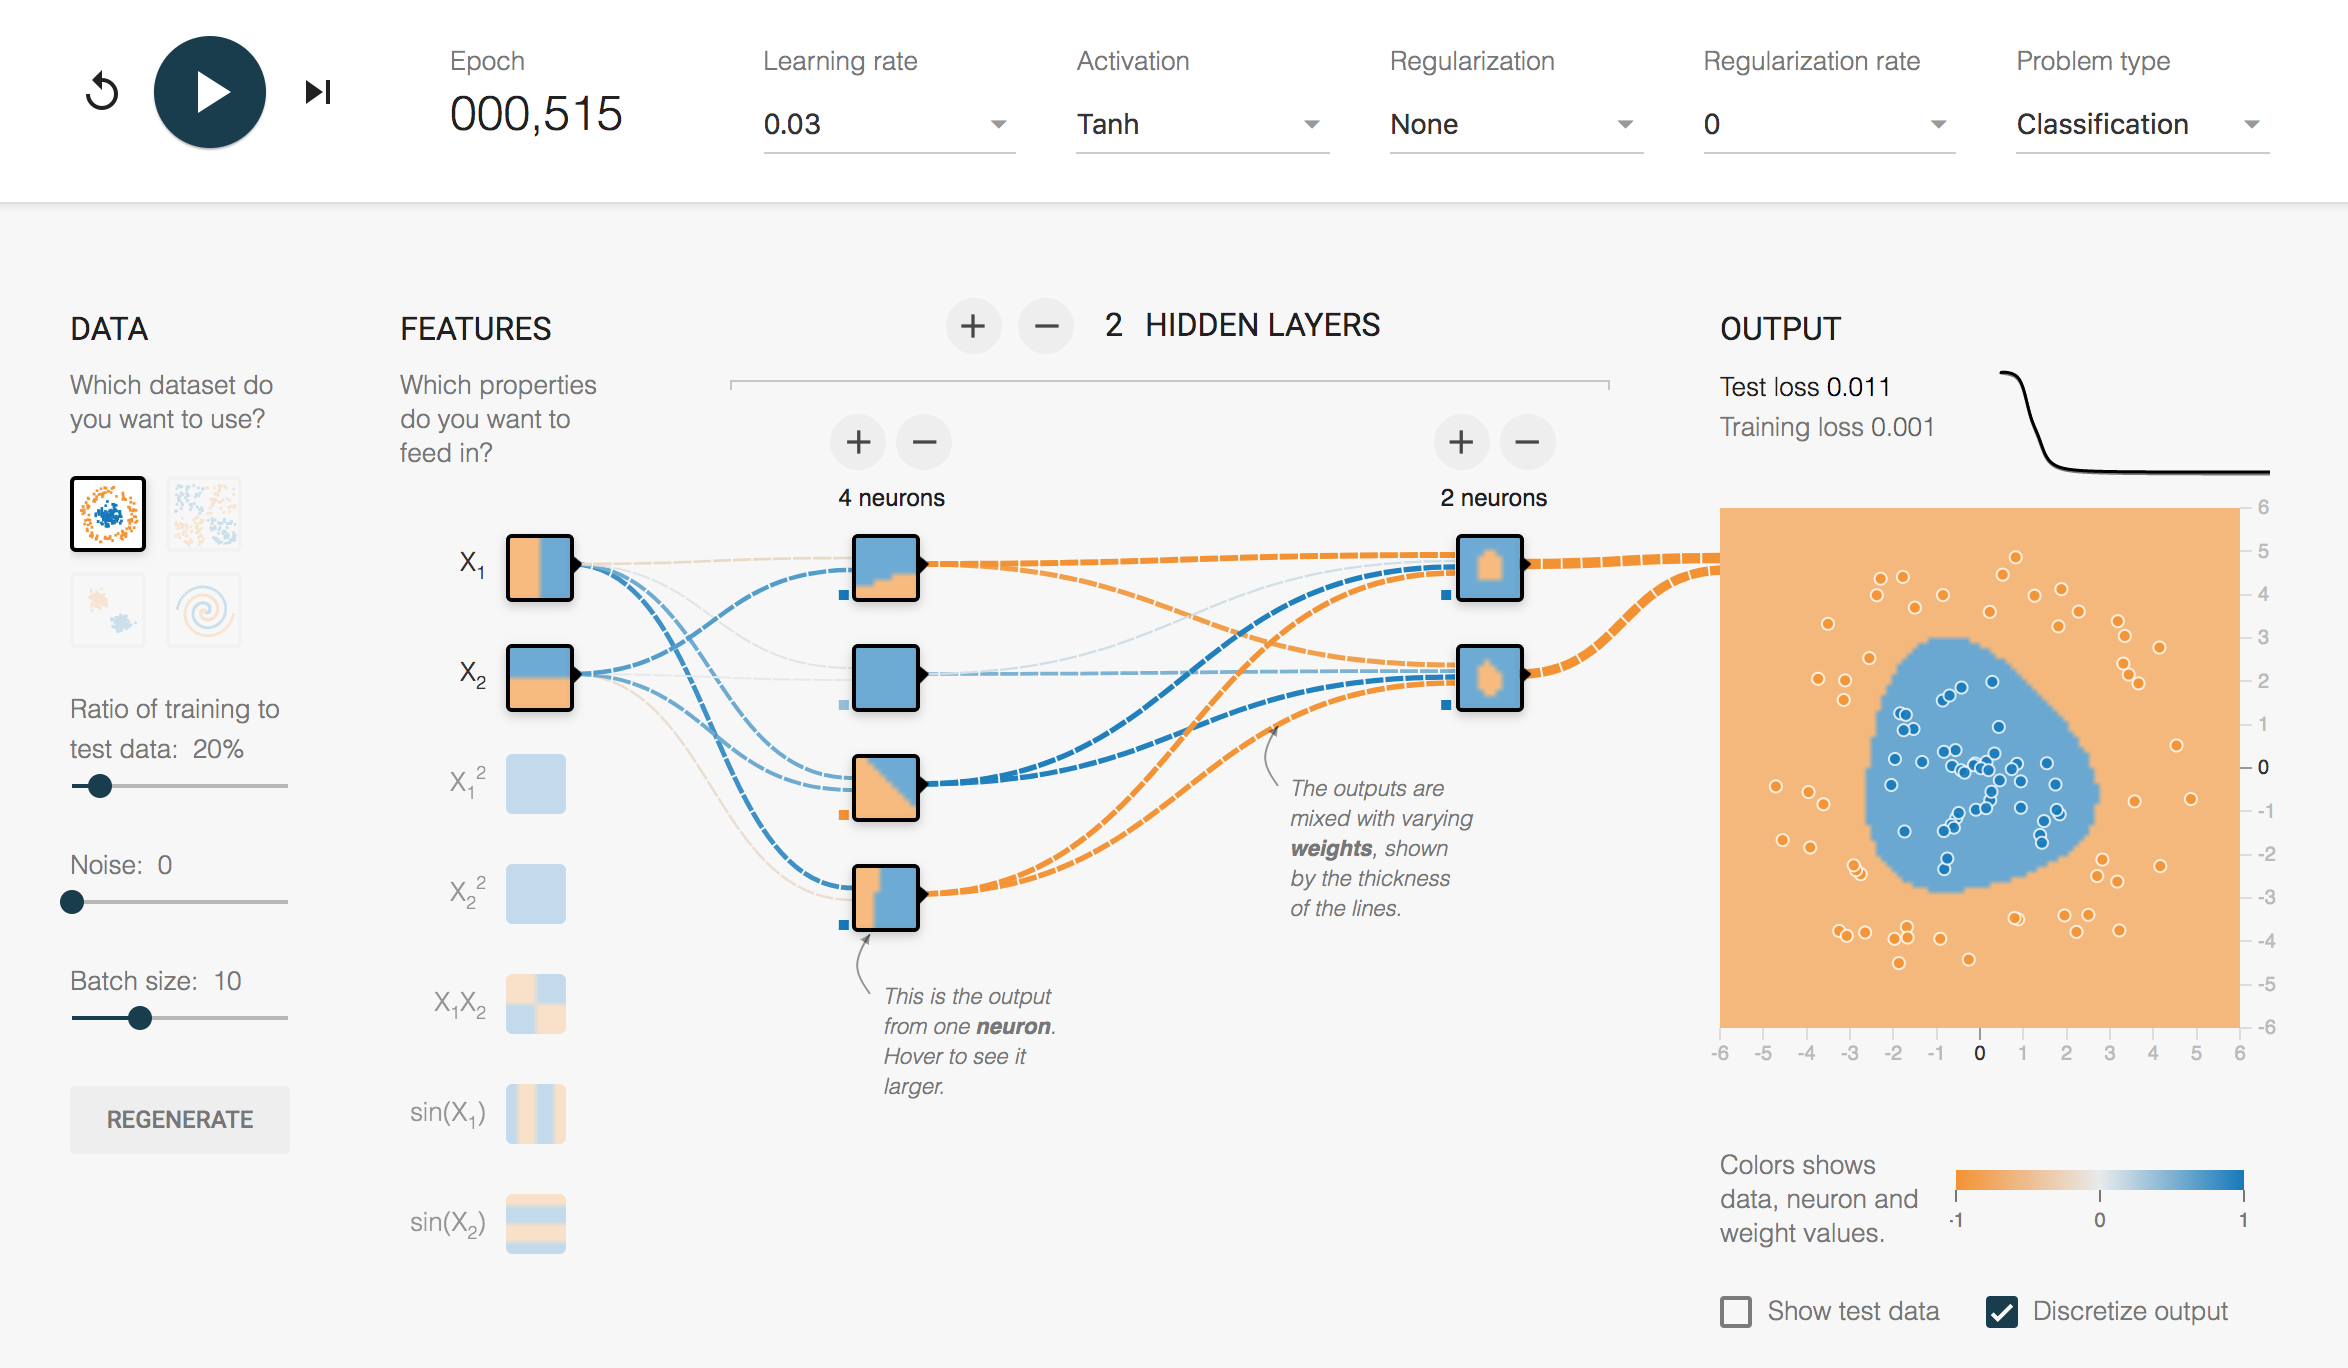
\includegraphics[scale=0.17]{tensorflow_demo.png}
\end{center} 

Голубым цветом обозначен первый класс, рыжим второй. Внутри каждого нейрона визуализирована та разделяющая поверхность, которую он выстраивает. Так, первый слой ищет разделяющую линию. Второй слой пытается из этих линий выстроить более сложные фигуры и так далее. Чем ярче связь между нейронами, тем больше весовой коэффициент, относящейся к ней. Синие связи --- положительные, рыжие --- отрицательные. Чем тусклее связь, тем он ближе к нулю. 

Маша заметила, что с её получившейся архитектурой что-то не так. Какие проблемы вы в ней видите?
\end{problem} 

\begin{sol}
Нейросетка Маши оказалась избыточной. Во-первых, можно увидеть, что на первом слое есть нейрон, который вообще ничего не делает. Связи, которые идут к нему от входов настолько тусклые (коэффициенты при них равны нулю), что их даже не видно на картинке. От этого нейрона смело можно избавиться и сделать архитектуру проще. 

Во-вторых, можно заметить, что на последнем слое у нас есть два одинаковых нейрона. Один из них смело можно выбрасывать. 

\begin{center} 
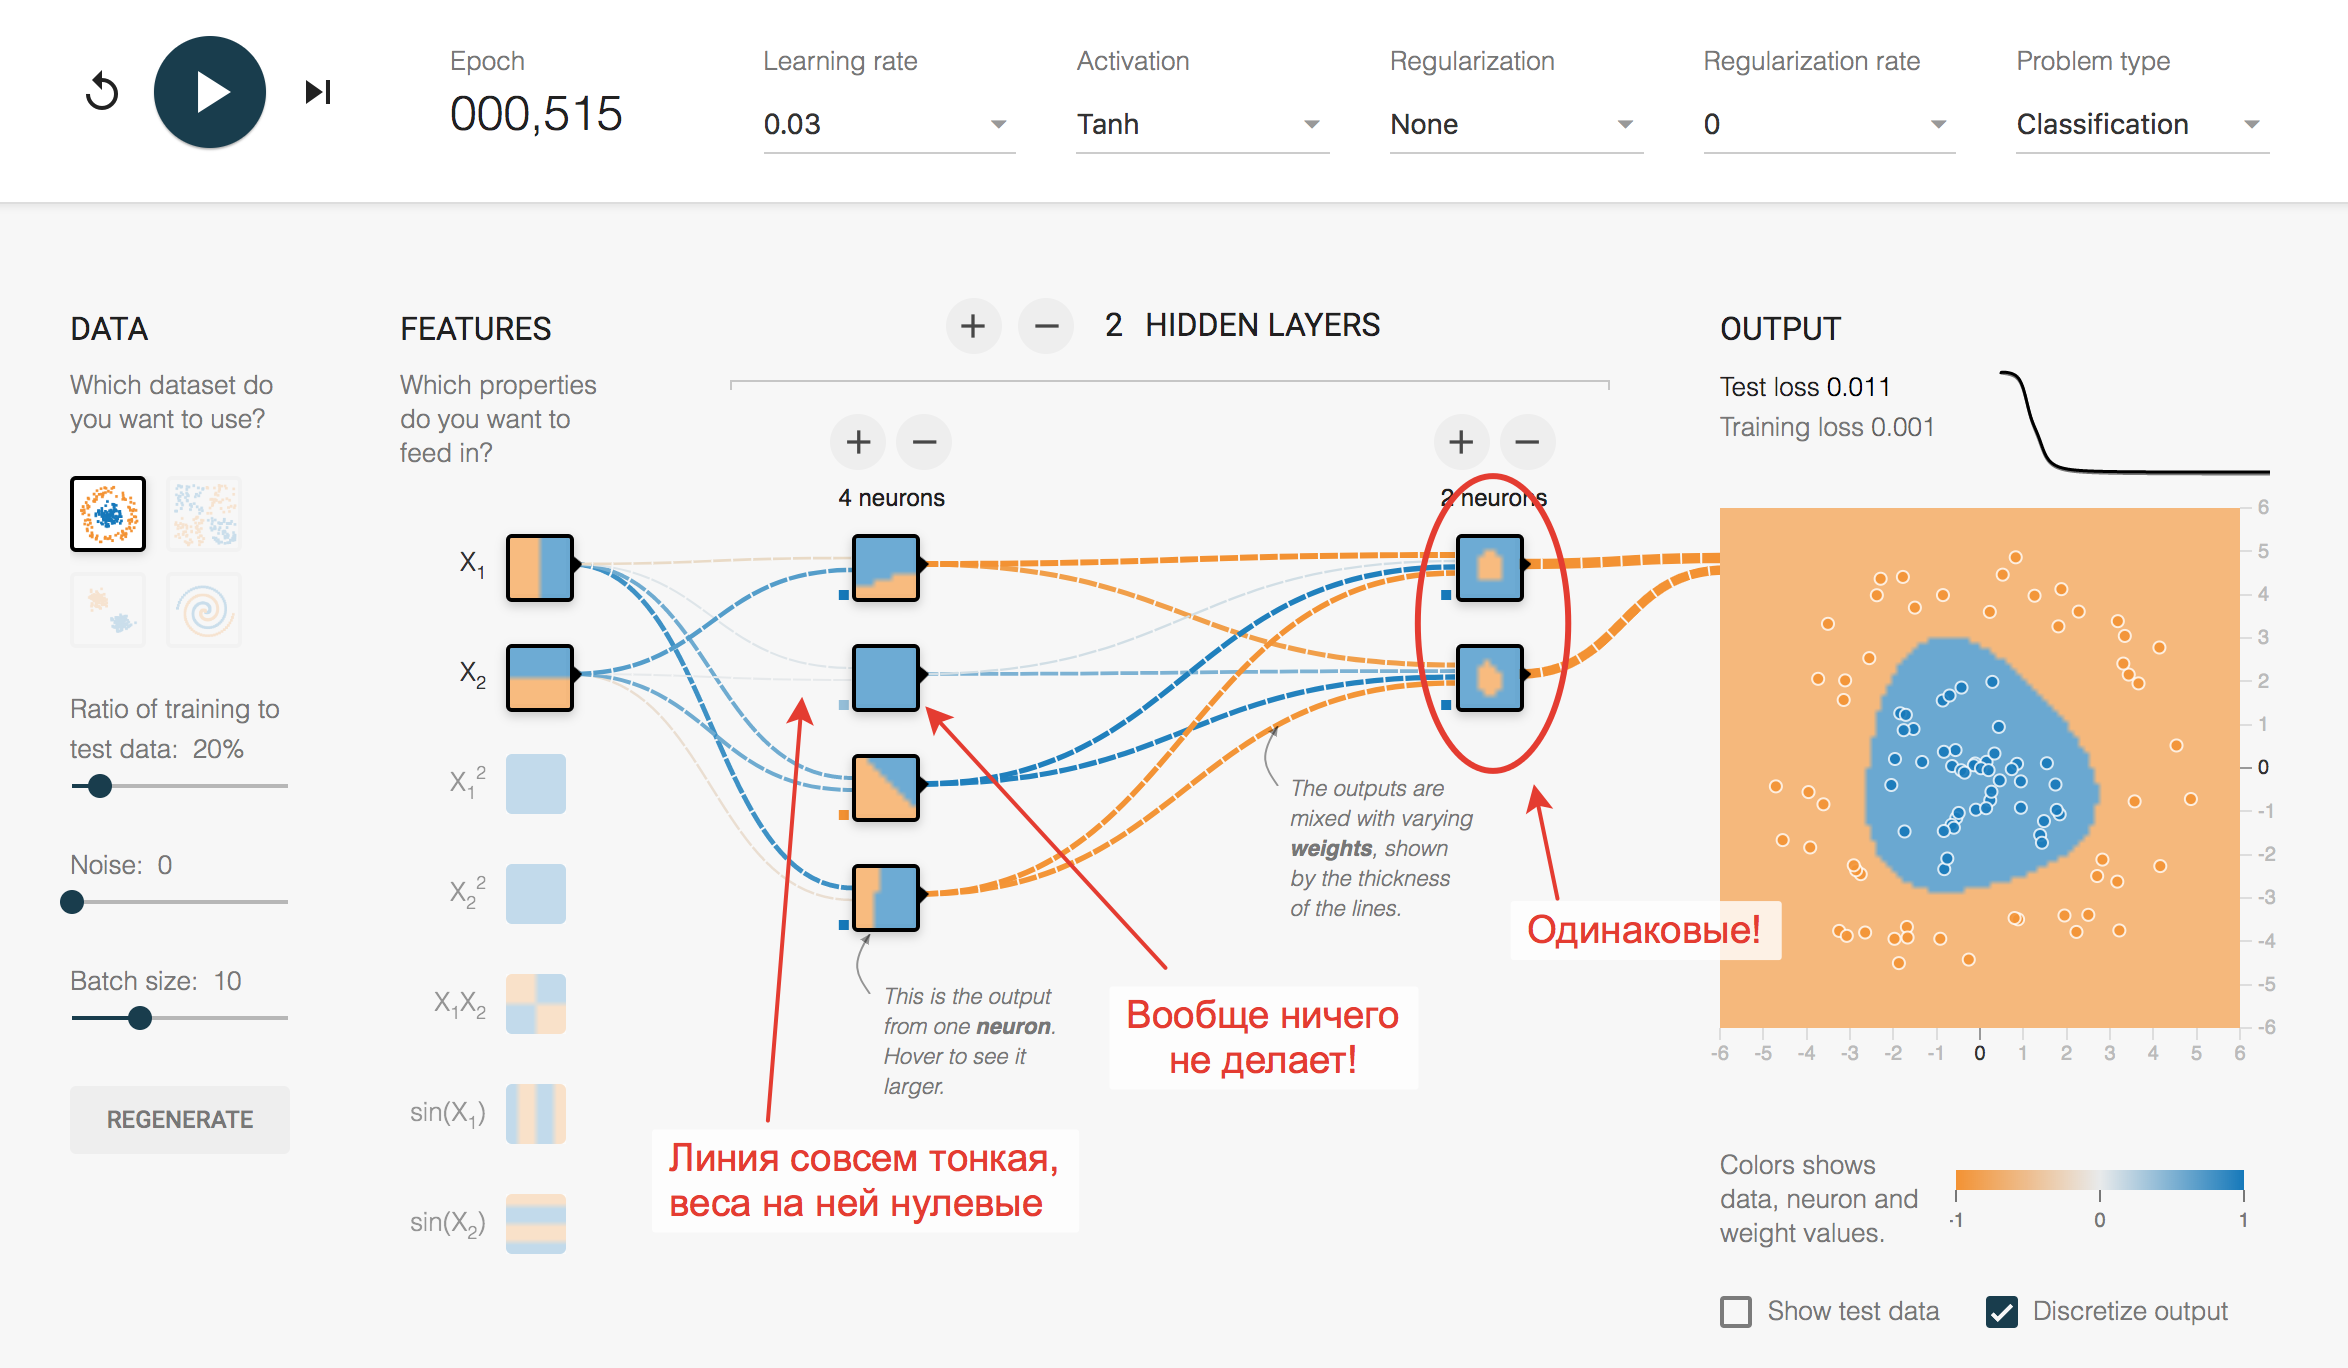
\includegraphics[scale=0.17]{tensorflow_demo2.png}
\end{center} 


Для решения такой простой задачи классификации подойдёт более простая модель. Сколько минимально нужно нейронов, чтобы её решить вам и Маше предстоит выяснить в следующей задачке. 
\end{sol}


%%%-------------------------------------------
\begin{problem}{(минималочка)}
Сколько минимально нейронов необходимо для решения следующих задач классификации?  Сколько слоёв минимально должно быть в нейросетке?  Почему?  

\begin{minipage}{0.3\linewidth} 
\begin{center}
\begin{tikzpicture}[scale = 0.7, line cap=round,line join=round,x=1.0cm,y=1.0cm]
	\draw [fill=red] (-2.6,4.9) circle (2.5pt);
	\draw [fill=red] (-2.,4.) circle (2.5pt);
	\draw [fill=red] (-1.42,4.9) circle (2.5pt);
	\draw [fill=blue] (-0.44,5.84) circle (2.5pt);
	\draw [fill=blue] (-1.52,5.9) circle (2.5pt);
	\draw [fill=blue] (-3.,6.) circle (2.5pt);
	\draw [fill=blue] (-4.02,5.7) circle (2.5pt);
	\draw [fill=blue] (-3.36,4.28) circle (2.5pt);
	\draw [fill=blue] (-2.4,2.92) circle (2.5pt);
	\draw [fill=blue] (-1.18,3.38) circle (2.5pt);
	\draw [fill=blue] (-0.56,4.16) circle (2.5pt);
	\draw [fill=blue] (0.,5.) circle (2.5pt);
	\draw [fill=blue] (-3.52,3.32) circle (2.5pt);
	\draw [fill=blue] (-0.44,2.5) circle (2.5pt);
	\draw [fill=blue] (-1.44,2.78) circle (2.5pt);
	\draw [fill=blue] (0.06,6.38) circle (2.5pt);
	\draw [fill=blue] (-2.96,6.78) circle (2.5pt);
	\draw [fill=blue] (-4.02,4.56) circle (2.5pt);
	\draw [fill=red] (-2.06,4.62) circle (2.5pt);
	\draw [fill=red] (-2.,5.) circle (2.5pt);
	\draw [fill=red] (-1.72,4.4) circle (2.5pt);
	\draw [fill=red] (-2.46,4.42) circle (2.5pt);
	\draw [fill=blue] (-2.22,6.26) circle (2.5pt);
\end{tikzpicture}
\end{center} 
\end{minipage} 
\hfill
\begin{minipage}{0.3\linewidth} 
\begin{center}
\begin{tikzpicture}[scale = 0.7, line cap=round,line join=round,x=1.0cm,y=1.0cm]
	\draw [fill=blue] (1.84,5.84) circle (2.5pt);
	\draw [fill=blue] (1.84,4.86) circle (2.5pt);
	\draw [fill=blue] (1.84,3.62) circle (2.5pt);
	\draw [fill=blue] (1.84,2.62) circle (2.5pt);
	\draw [fill=blue] (2.68,2.56) circle (2.5pt);
	\draw [fill=blue] (2.68,3.38) circle (2.5pt);
	\draw [fill=blue] (2.54,4.5) circle (2.5pt);
	\draw [fill=blue] (2.64,5.72) circle (2.5pt);
	\draw [fill=blue] (5.04,5.6) circle (2.5pt);
	\draw [fill=blue] (5.,4.56) circle (2.5pt);
	\draw [fill=blue] (4.92,3.36) circle (2.5pt);
	\draw [fill=blue] (4.92,2.48) circle (2.5pt);
	\draw [fill=blue] (5.98,2.32) circle (2.5pt);
	\draw [fill=blue] (5.98,3.16) circle (2.5pt);
	\draw [fill=blue] (6.,4.) circle (2.5pt);
	\draw [fill=blue] (5.94,4.76) circle (2.5pt);
	\draw [fill=blue] (5.92,5.34) circle (2.5pt);
	\draw [fill=red] (3.42,5.12) circle (2.5pt);
	\draw [fill=red] (3.44,5.94) circle (2.5pt);
	\draw [fill=red] (4.28,5.8) circle (2.5pt);
	\draw [fill=red] (4.28,5.3) circle (2.5pt);
	\draw [fill=red] (3.54,3.98) circle (2.5pt);
	\draw [fill=red] (4.,4.) circle (2.5pt);
	\draw [fill=red] (3.5,2.98) circle (2.5pt);
	\draw [fill=red] (4.18,2.94) circle (2.5pt);
	\draw [fill=red] (3.4,2.32) circle (2.5pt);
	\draw [fill=red] (4.18,2.36) circle (2.5pt);
	\draw [fill=red] (3.98,4.56) circle (2.5pt);
\end{tikzpicture}
\end{center} 
\end{minipage} 

\todo[inline]{Добавить норм ксор для точек как на семе} 
\end{problem}

\begin{sol}

\end{sol} 


%%%-------------------------------------------
\begin{problem}{(универсальный регрессор)}
Доказать, что с помощью однослойной нейронной сетки можно приблизить любую непрерывную функцию от одного аргумента $f(x)$ со сколь угодно большой точностью\footnote{\url{http://neuralnetworksanddeeplearning.com/chap4.html}}.  

\textbf{Hint:}  Вспомните, что любую непрерывную функцию можно приблизить с помощью кусочно-линейной функции (ступеньки). Осознайте как с помощью пары нейронов можно описать такую ступеньку. Соедините все ступеньки в сумму с помощью выходного нейрона. 
\end{problem}

\begin{sol}

\end{sol} 


\section{50 оттенков градиентного спуска}

%\epigraph{ }{ }

%%%-------------------------------------------


\section{Backpropagation}

%\epigraph{ }{ }

Что происходит, когда мы суём пальцы в розетку? Нас бьёт током! Мы делаем ошибку, и она распространяется по нашему телу назад. 


%%%-------------------------------------------
\begin{problem}{(граф вычислений)}
	Изобразите для функции  $f(x,y) = x^2 + xy + (x + y)^2$ граф вычислений. Найдите производные всех выходов по всем входам. Опираясь на граф выпишите частные производные функции $f$.\footnote{По мотивам книги Николенко "Глубокое обучение" (стр. 79)}
\end{problem} 


%%%-------------------------------------------
\begin{problem}{(придумываем backpropagation)}
	Дана нейросетка: 
\begin{center}
	\begin{tikzpicture}[line cap=round,line join=roundx=1.0cm,y=1.0cm]
	\clip(-3.68,0.12) rectangle (12.02,4.76);
	\draw [line width=2.pt] (-2.56,1.54) circle (0.5215361924162121cm);
	\draw [line width=2.pt] (-2.5,3.5) circle (0.5215361924162117cm);
	\draw [line width=2.pt] (0.,4.)-- (2.,4.);
	\draw [line width=2.pt] (2.,4.)-- (2.,3.);
	\draw [line width=2.pt] (2.,3.)-- (0.,3.);
	\draw [line width=2.pt] (0.,3.)-- (0.,4.);
	\draw [line width=2.pt] (0.,2.)-- (2.,2.);
	\draw [line width=2.pt] (2.,2.)-- (2.,1.);
	\draw [line width=2.pt] (2.,1.)-- (0.,1.);
	\draw [line width=2.pt] (0.,1.)-- (0.,2.);
	\draw [line width=2.pt] (4.,4.)-- (6.,4.);
	\draw [line width=2.pt] (6.,4.)-- (6.,3.);
	\draw [line width=2.pt] (6.,3.)-- (4.,3.);
	\draw [line width=2.pt] (4.,3.)-- (4.,4.);
	\draw [line width=2.pt] (4.,2.)-- (6.,2.);
	\draw [line width=2.pt] (6.,2.)-- (6.,1.);
	\draw [line width=2.pt] (6.,1.)-- (4.,1.);
	\draw [line width=2.pt] (4.,1.)-- (4.,2.);
	\draw [line width=2.pt] (8.,3.)-- (10.,3.);
	\draw [line width=2.pt] (10.,3.)-- (10.,2.);
	\draw [line width=2.pt] (10.,2.)-- (8.,2.);
	\draw [line width=2.pt] (8.,2.)-- (8.,3.);
	\draw [line width=2.pt] (-1.9787961021013818,3.4813855750750493)-- (0.,3.48);
	\draw [line width=2.pt] (-1.9787961021013818,3.4813855750750493)-- (0.,1.36);
	\draw [line width=2.pt] (-2.039699677075342,1.5041172191086443)-- (0.,1.36);
	\draw [line width=2.pt] (-2.039699677075342,1.5041172191086443)-- (0.,3.48);
	\draw [line width=2.pt] (2.,3.54)-- (4.,3.54);
	\draw [line width=2.pt] (2.,1.48)-- (4.,1.48);
	\draw [line width=2.pt] (2.,1.48)-- (4.,3.54);
	\draw [line width=2.pt] (2.,3.54)-- (4.,1.48);
	\draw [line width=2.pt] (6.,3.5)-- (8.,2.46);
	\draw [line width=2.pt] (6.,1.46)-- (8.,2.46);
	\draw (4.54, 3.75) node[anchor=north west] {$f(t)$};
	\draw (4.54,1.8) node[anchor=north west] {$f(t)$};
	\draw (0.52, 3.75) node[anchor=north west] {$f(t)$};
	\draw (0.54, 1.8) node[anchor=north west] {$f(t)$};
	\draw (8.6, 2.8) node[anchor=north west] {$f(t)$};
	\draw (-2.8, 1.8) node[anchor=north west] {$x_2$};
	\draw (-2.8, 3.75) node[anchor=north west] {$x_1$};
	\draw (6.78,3.8) node[anchor=north west] {$w_1^3$};
	\draw (6.76,2) node[anchor=north west] {$w_{2}^3$};
	\draw (-1.3,4.4) node[anchor=north west] {$w_{11}^1$};
	\draw (-1.5,2.2) node[anchor=north west] {$w_{21}^1$};
	\draw (-1.52,3.55) node[anchor=north west] {$w_{12}^1$};
	\draw (-1.58,1.4) node[anchor=north west] {$w_{22}^1$};
	\draw (2.76,4.4) node[anchor=north west] {$w_{11}^2$};
	\draw (2.68,1.4) node[anchor=north west] {$w_{22}^2$};
	\draw (2.52,2.25) node[anchor=north west] {$w_{21}^2$};
	\draw (2.48,3.55) node[anchor=north west] {$w_{12}^2$};
	\draw (10.5, 2.8) node[anchor=north west] {$y$};
	\end{tikzpicture}
\end{center}	
	\begin{enumerate}
		\item  Перепишите её как сложную функцию. 
		
		\item Запишите эту функцию в матричном виде.
		
		\item  Предположим, что $L(W_1,W_2,W_3) = \frac{1}{2} \cdot (y - \hat y)^2$ --- функция потерь, где $W_i$ --- веса $i-$го слоя.  Найдите производную функции $L$ по всем весам $W_i$. 
		
		\item Выглядит не очень оптимально, правда? Выпишите все производные в том виде, в котором их было бы удобно использовать для алгоритма обратного распространения ошибки, а затем, сформулируйте сам алгоритм.
	\end{enumerate}
\end{problem}


%%%-------------------------------------------
\begin{problem}{(backpropagation руками)}
	Как-то раз Вовочка решал задачу классификации. С тех пор у него в кармане завалялась нейросеть: 
	\begin{center}
		\begin{tikzpicture}[scale = 1.5, line cap=round,line join=round,x=1.0cm,y=1.0cm]
		\clip(-4.624679143882289,1.3686903642723092) rectangle (3.8521836267384844,4.8154607149701345);
		\draw [line width=2.pt] (-2.5,2.5) circle (0.5cm);
		\draw [line width=2.pt] (-0.5,2.5) circle (0.5cm);
		\draw [line width=2.pt] (1.5,2.5) circle (0.5cm);
		\draw [->,line width=2.pt] (-3.5,4.) -- (-2.831496141146421,2.874313115459547);
		\draw [->,line width=2.pt] (-4.,2.5) -- (-3.,2.5);
		\draw [->,line width=2.pt] (-2.,2.5) -- (-1.,2.5);
		\draw [->,line width=2.pt] (0.,2.5) -- (1.,2.5);
		\draw [->,line width=2.pt] (2.,2.5) -- (3.,2.5);
		\draw [->,line width=2.pt] (-1.5,4.) -- (-0.8294354120380936,2.8761280490674572);
		\draw [->,line width=2.pt] (0.5,4.) -- (1.1775032003746246,2.8820939861230355);
		\draw (-3.686865302879703,4.5) node[anchor=north west] {$1$};
		\draw (-1.67726421501702,4.5) node[anchor=north west] {$1$};
		\draw (0.2957986712481599,4.5) node[anchor=north west] {$1$};
		\draw (-4.320194130569761,2.805859627107445) node[anchor=north west] {$x$};
		\draw (3.1214195947884176,2.7693214255099416) node[anchor=north west] {$y$};
		\draw (-3.7112241039447054,3.07380643882247) node[anchor=north west] {$w_1^1$};
		\draw (-3.114433477852151,3.9750820782275555) node[anchor=north west] {$w_0^1$};
		\draw (-1.7138024166145234,3.122524040952475) node[anchor=north west] {$w_1^2$};
		\draw (-1.1535499921194723,4.13341428515007) node[anchor=north west] {$w_0^2$};
		\draw (1.0387421037307276,4.109055484085068) node[anchor=north west] {$w_0^3$};
		\draw (0.2836192707156588,3.0859858393549713) node[anchor=north west] {$w_1^3$};
		\end{tikzpicture}
	\end{center} 
	
	В качестве функции активации используется сигмоид: $f(t) = \frac{e^t}{1 + e^t}$.  Есть два наблюдения: $x_1 = 1, x_2 = 5$, $y_1 =1$, $y_2 = 0$. Скорость обучения $\gamma = 1$. В качестве инициализации взяты нулевые веса. Как это обычно бывает, Вовочка обнаружил её в своих штанах после стирки и очень обрадовался.  Теперь он собирается сделать два шага стохастического градиентного спуска, используя алгоритм обратного распространения ошибки. Помогите ему. 
\end{problem}


%%%-------------------------------------------
\begin{problem}{(ещё один backpropagation)}
	Пусть у нас есть нейронка: 
	
	$$ 
	y = f(X \cdot W_2 ) \cdot W_1 
	$$
	
	Как для функции потерь $L(W_1, W_2) = (y - \hat y)^2$ будет выглядеть алгоритм обратного распространения ошибки, если $f(t) = ReLU(t) =  \max(0; t)$? Найдите все выходы, все промежуточные производные.  Опишите правило, по которому производная будет накапливаться, а также сам шаг градиентного спуска. 
\end{problem} 


\begin{problem}
	Маша (ОПЯТЬ ОНА?!) собрала нейросеть: 
	
	\begin{equation*}
	y =   \max \left( 0;  X \cdot  \begin{pmatrix} 1 & -1 \\ 0.5 & 0 \end{pmatrix} \right) \cdot \begin{pmatrix} 0.5 \\ 1 \end{pmatrix} 
	\end{equation*}

	Теперь Маша внимательно смотрит на неё.
	
	\begin{enumerate}
		\item  Первый слой нашей нейросетки --- линейный. По какой формуле делается forward pass? Предположим, что на вход пришло наблюдение $x = (1, 2)$. Сделайте через этот слой forward pass и найдите выход из слоя.
		
		\item Найдите для первого слоя производную выхода по входу. При обратном движении по нейросетке, в первый слой пришёл накопленный градиент $(-1, 0)$. Каким будет новое накопленное значение градиента, которое выплюнет из себя линейный слой? 
		
		\item Второй слой нейросетки ---- функция активации, $ReLU.$  По какой формуле делается forward pass? На вход в него поступило значение $(2, -1)$. Сделайте через него forward pass. 
		
		\item Найдите для второго слоя производную выхода по входу. При обратном движении по нейросетке во второй слой пришёл накопленный градиент $(-1, -2)$.  Каким будет новое накопленное значение градиента, которое выплюнет из себя $ReLU$? 
		
		\item Третий слой нейросетки --- линейный.  По какой формуле делается forward pass? Пусть на вход поступило значение $(2,0)$.  Сделайте через него forward pass. 
		
		\item Найдите для третьего слоя производную выхода по входу. При обратном движении по нейросетке, в третий слой пришёл накопленный градиент $-2$. Каким будет новое накопленное значение градиента, которое выплюнет из себя линейный слой? 
		
		\item Мы решаем задачу Регрессии. В качестве функции ошибки мы используем $MSE$. Пусть для рассматриваемого наблюдения реальное значение $y = 0$. Найдите значение $MSE$. Чему равна производная $MSE$ по входу (прогнозу)? Каким будет накопленное значение градиента, которое $MSE$ выплюнет из себя в предыдущий слой нейросетки, если изначально значение градиента инициализированно единицей? 
		
		\item Пусть скорость обучения $\gamma = 1$.  Сделайте для весов нейросети шаг градиентного спуска. 
	\end{enumerate}

		Посидела Маша, посидела, и поняла, что неправильно она всё делает. В реальности перед ней не задача регрессии, а задача классификации. 
	
	\begin{enumerate}	
		\item Маша навинтила поверх второго линейного слоя сигмоиду. Как будет для неё выглядеть forward pass? Сделайте его. Найдите для сигмоиды производную выхода по входу.
		
		\item В качестве функции потерь Маша использует $logloss.$ Как для этой функции потерь выглядит forward pass? Сделайте его. Найдите для $logloss$ производную выхода по входу. 
		
		\item Как будет выглядеть backward pass через $logloss$ и сигмоиду? Прделайте его. Как изменится процедура градиентного спуска для остальной части сети? 
	\end{enumerate}

\end{problem} 





\section{Активация} 

%\epigraph{ }{ }

% Тут пара задач на освоиться с softmax и logloss 
\begin{problem}
	У Бандерлога три наблюдения\footnote{Про другие приключения Бандерлога читай тут: \url{https://github.com/bdemeshev/mlearn_pro/blob/master/mlearn_pro.pdf}}, первое наблюдение — кит, остальные — муравьи. Киты кодируются $y_i = 1$, муравьи — $y_i = 0$.  В качестве регрессоров Бандерлог берёт номера наблюдений $x_i = i$.  После этого Бандерлог оценивает логистическую регрессию с константой.
	
	\begin{enumerate}
		\item Выпишите эмпирическую функцию риска, которую минимизирует Бандерлог;
		\item При каких оценках коэффициентов логистической регрессии эта функция достигает своего минимума?
	\end{enumerate}
\end{problem}



\begin{problem}{ }
Та, в чьих руках находится лёрнинг (это Маша), решила немного поэкспериментировать с выходами из своей сетки. 
\begin{itemize}
	\item[a)]  Для начала Маша решила, что хочет решать задачу классификации на два класса и получать на выходе вероятность принадлежности к первому. Что ей надо сделать с последним слоем сетки? 
	\item[b)]  Теперь Маша хочет решать задачу классификации на $K$ классов. Что ей делать с последним слоем? 
	\item[c)]  Новые вводные! Маша хочет спрогнозировать рейтинг фильма на "Кинопоиске". Он измеряется по шкале от $0$ до $10$ и принимает любое непрерывное значение. Как Маша может приспособить для этого свою нейронку? 
	\item[d)]  У Маши есть куча новостей. Каждая новость может быть спортивной, политической или экономической. Иногда новость может относится сразу к нескольким категориям. Как Маше собрать нейросетку для решения этой задачи?  Как будет выглядеть при этом функция ошибки? 
	\item[e)]  Маша пошла в кафе. А там куча народу. Сейчас она сидит за столиком, попивает ванильный топлёный кортадо и думает о нём, о лёрнинге.  Сейчас мысль такая: как можно спрогнозировать число людей в кафе так, чтобы на выходе сетка всегда прогнозировала целое число. Надо ли как-то при этом менять функцию потерь? 
	% \item[f)] Пункт с регрессией и весами из денег 
\end{itemize}
\end{problem}


\begin{problem}
	Бандерлог чуть внимательнее присмотрелся к своему третьему наблюдению и понял, что это не кит, а бобёр. Теперь ему нужно решать задачу классификации на три класса. Он решил использовать для этого нейросеть с softmax-слоем на выходе.  Предположим, что сетка обучилась и на двух новых наблюдениях, перед самым softmax-слоем она выплюнула $1, 2, 5$ и $2, 5, 1$.
	
	\begin{enumerate}
		\item Чему равны вероятности получить кита, муравья и бобра для обеих ситуаций? 
		\item Пусть первым был кит, а вторым бобёр.  Чему будет равна logloss-ошибка? 
	\end{enumerate}
\end{problem}

\begin{problem}
	Иногда в функцию Softmax добавляют дополнительный параметр $T$, который называют температурой. Тогда она приобретает вид 
	
	\[ 
	f(z) =  \frac{e^{\tfrac{z_i}{T}}}{ \sum_{k=1}^K e^{\tfrac{z_k}{T}}}
	\]

	Обычно это делается, когда с помощью нейросетки нужно сгенерировать какой-нибудь новый объект.  Пусть у нас есть три класса. Наша нейросеть выдала на последнем слое числа $1,2,5$. 

	\begin{enumerate}
		\item  Какое итоговое распределение вероятностей мы получим, если $T = 10$? 
		\item  А если $T = 1$? 
		\item  А если $T = 0.1$? 
		\item  Какое распределение получится при $T \to 0$? 
		\item  А при $T \to \infty$? 
		\item  Предположим, что объектов на порядок больше. Например, это реплики, которые Алиса может сказать вам в ответ на какую-то фразу.  Понятное дело, что вашей фразе будет релевантно какое-то подмножество ответов. Какое значение температуры сэмплирования $T$ смогут сделать реплики Алисы непредсказуемыми? А какие сделают их однотипными? 
	\end{enumerate}
\end{problem}


\begin{problem}
	Функция $f(t) = \frac{e^t}{1 + e^t}$ называется сигмоидой\footnote{В этом всём тоже замешан один Бандерлог.}.
	
		\begin{enumerate}
		\item Что происходит при $t \to +\infty$? А при $t \to -\infty$?
		\item Как связаны между собой $f(t)$ и  $f(-t)$?
		\item Как связаны между собой $f'(t)$ и  $f'(-t)$?
		\item Как связаны между собой $f(t)$ и $f'(t)$? 
		\item Найдите $f(0)$, $f'(0)$ и $\ln f(0)$.
		\item Найдите обратную функцию $f^{-1}(t)$
		\item Как связаны между собой $\frac{d\ln f(t)}{dt}$ и $f(-t)$?
		\item Постройте графики функций $f(t)$ и $f'(t)$.
		\item Разложите $h(\beta_1, \beta_2)=\ln f(y_i(\beta_1 + \beta_2 x_i))$ в ряд Тейлора до второго порядка в окрестности точки $\beta_1=0$, $\beta_2=0$.
	\end{enumerate}
\end{problem} 


\section{Регуляризаторы}

%\epigraph{ }{ }

% \begin{problem}
% 	Маша услышала про машин лёрнинг и решила, что они и есть та самая Маша, которой этот лёрнинг принадлежит. Теперь она собирается обучить нейронную сеть для решения задачи регрессии, На вход в неё идёт $12$ переменных, в сетке есть $3$ скрытых слоя. В пером слое $300$ нейронов, во втором $200$, в третьем $100$. 
	
% 	\begin{itemize}
% 		\item[a)] Сколько параметров предстоит оценить Маше?  Сколько наблюдений вы бы на её месте использовали? 
% 		\item[b)] Пусть в каждом слое была отключена половина нейронов. Сколько коэффициентов необходимо оценить?
% 		\item[c)] Предположим, что Маша решила после первого слоя добавить в свою сетку Dropout c вероятностью $p$.  Какова вероятность того, что отключится весь слой? 
% 		\item[d)] Маша добавила Dropout c вероятностью $p$. после каждого слоя. Какова вероятность того, что один из слоёв отключится и сетка не сможет учиться? 
% 		\item[e)] Пусть случайная величина $N$ --- это число включённых нейронов. Найдите её математическое ожидание и дисперсию. Если Маша хочет проредить сетку на четверть, какое значение $p$ она должна поставить? 
% 		\item[f)] Пусть случайная величина $P$ --- это число параметров в нейросети, которое необходимо оценить. Найдите её математическое ожидание и дисперсию. Почему найденное вами математическое ожидание выглядит очень логично? Что оно вам напоминает? Обратите внимание на то, что смерть одного из параметров легко может привести к смерти другого.
% 	\end{itemize}
% \end{problem}


% %\begin{problem}
% %  Сделать задачу по связи ранней остановки и регуляризатора 
% %\end{problem}

% \section*{Ещё задача}

% Если вы никогда не решали эту задачку, рекомендую сделать это. Она довольно неплохо открывает чакру на работу с регуляризаторами, и показывает как именно они стягивают к нулю коэффициенты, не давая модели переобучаться. В рамках нейросеток механизм точно такой же. 

% \begin{problem}
% 	Вася измерил вес трёх покемонов,  $y_1=6$, $y_2=6$, $y_3=10$.  Вася хочет спрогнозировать вес следующего покемона. Модель для веса покемонов у Васи очень простая, $y_i = \beta + \varepsilon_i$, поэтому прогнозирует Вася по формуле $\hat y_i = \hat \beta$.
	
% 	Для оценки параметра $\beta$ Вася использует следующую целевую функцию:
	
% 	\[
% 	\sum (y_i - \hat \beta)^2 + \lambda \cdot \hat \beta^2
% 	\]
	
% 	\begin{enumerate}
% 		\item[a)] Найдите оптимальное $\hat \beta$ при $\lambda =0$.
% 		\item[б)] Найдите оптимальное $\hat \beta$ при произвольном $\lambda$. Правда ли, что чем больше $\lambda$, тем меньше $\beta$? 
% 		\item[в)] Подберите оптимальное $\lambda$ с помощью кросс-валидации leave one out («выкинь одного»). При такой валидации на первом шаге мы оцениваем модель на всей выборке без первого наблюдения, а на первом тестируем её. На втором шаге мы оцениваем модель на всей выборке без второго наблюдения, а на втором тестируем её. И так далее $n$ раз. Каждое наблюдение является отдельным фолдом.
% 		\item[г)] Найдите оптимальное $\hat \beta$ при $\lambda_{CV}$.
% 	\end{enumerate}
% \end{problem}

% \begin{problem}
% Есит нейрон с ReLU в качестве инициализации используется распределение ко-ко-ко. С какой вероятностью нейрон умрёт сразу же при инициализации? Какое распределение и с какими параметрами надо использовать, чтобы этого не произошло? Сюда же про инициализацию Хе.
% \end{problem}

% родить задачу из статьи dropout vs batchnorm

% задача на бачнорм из лекций воронцова


\section{Всего лишь кубики LEGO} 

%\epigraph{ }{ }

% сюда tasks6, LSTM, w2v и тп

% упражнение про разные модные виды ячеек типа резнетов и тп

\section{Итоговый тест в стел Носко}

\begin{enumerate} 
\item Вопрос про батчнормализацию первым слоем вместо нормализации в предобработке. 

\end{enumerate}






% \begin{center}
% \begin{tikzpicture}[scale = 1.5, line cap=round,line join=round,x=1.0cm,y=1.0cm]

% \node at (-1,2) {Схема матстата:}

% \path (-1,0) node(x) {\Huge $\hat \theta$} (3,0) node(y) {\Huge $f_{\hat \theta} (t)$};

% \node at (8, 0) {\footnotesize
%     \begin{varwidth}{\linewidth}\begin{itemize}
%         \item прогнозы
%         \item насколько точны прогнозы
%         \item ответы на вопросы (гипотезы)
%     \end{itemize}\end{varwidth}
% };

% \draw[->, line width=1.1pt] (-0.5,0) -- (2,0);
% \draw[->, line width=1.1pt] (4,0) -- (6,0);

% \node at (0.8, 1.6) { \footnotesize
%     \begin{varwidth}{\linewidth} \textbf{Хотим:}
%     \begin{itemize}
%         \item несмещённость: $E(\hat \theta) = \theta$
%         \item состоятельность: $\hat \theta \overset{p}{\to} \theta$
%         \item эффективность: дисперсия самая маленькая
%     \end{itemize}\end{varwidth}
% };

% \node at (-0.2, -1.45) { \footnotesize
%     \begin{varwidth}{\linewidth} \textbf{Cоюзники:}
%     \begin{itemize}
%         \item метод моментов
%         \item метод максимального \\ правдоподобия
%     \end{itemize}\end{varwidth}
% };

% \node at (3.5, -1.7) { \footnotesize
%     \begin{varwidth}{\linewidth} \textbf{Cоюзники:}
%     \begin{itemize}
%         \item ЦПТ
%         \item Дельта-метод
%         \item $\chi^2_n, t(n), F(n,m)$
%         \item Теорема Фишера
%     \end{itemize}\end{varwidth}
% };
% \end{tikzpicture}
% \end{center} 



\end{document}


